As mentioned in Chapter \ref{sec:cca}, in the sample starved regime where the number of
samples is less than the combined dimensions of the datasets, it is common to
regularize CCA. By adding a penalty to the $\ell_2$ norm of the canonical vectors in the
CCA objective function we arrive at a regularized version of CCA (RCCA). This optimization
also has a closed form solution that is dependent on the SVD of a matrix involving the
covariance matrices of our data. However, unlike CCA, in the samples starved regime, this
solution is tractable as all matrix inverses are well defined. 

In this section we explore the performance of empirical RCCA, which has been previously
unexplored. We investigate the effect that the regularization parameter has on the
correlation estimate of returned by RCCA. Similar to the analysis conducted in Chapter
\ref{sec:cca}, we compute empirical distributions of this correlation estimate generated
from datasets that contain a correlated signal and from datasets that are purely noise. We
then explore using the correlation estimate to detect the presence of a signal.

Motivated by ICCA, we then develop an informative version of RCCA (IRCCA) that only uses
the informative components of the provided datasets. Finally, we explore the performance
of IRCCA and compare it to that of RCCA. We are particularly interested in how the
regularization parameter affects the distributions of the correlation estimate. We compare
using these correlation estimates to detect the presence of a target signal given two
correlated datasets. Our analysis shows that IRCCA exhibits many attractive behaviors not
exhibited by RCCA.

\section{Mathematical Formulation of RCCA}
RCCA uses the same data assumptions as CCA as described in Section \ref{sec:cca_form}. The
objective is still to find the canonical vectors $\xI$ and $\xII$ that maximize the correlation
between the canonical variates $\wI=\xI^H\yI$ and $\wII=\xII^H\yII$. RCCA introduces a
regularization parameter, $\eta$, that penalizes the $\ell_2$ norm of the canonical
vectors. Formally, the RCCA optimization problem is
\begin{equation}\label{eq:rcca_opt1}
  \begin{aligned}
    &\argmax_{\xI,\xII}&&\rho = E[\wI\wII]\\
    & \text{subject to}&& E[\wI^2] + \eta \xI^H\xI\leq 1\\
    &&& E[\wI^2] + \eta \xII^H\xII\leq 1.\\
  \end{aligned}
\end{equation}
Note that in this formulation, we use the same regularization parameter for both canonical
vectors. One could relax this constraint and allow individual regularization parameters
$\eta_1$ and $\eta_2$ for each of the canonical vectors. 

Substituting the expressions for the canonical variates and correlation matrices used for
CCA, the RCCA optimization problems may be written
\begin{equation}\label{eq:rcca_opt2}
  \begin{aligned}
    &\argmax_{\xI,\xII}&&\rho = \xI^H\RIII\xII\\
    & \text{subject to}&& \xI^H\RI\xI + \eta \xI^H\xI\leq 1\\
    &&& \xII^H\RII\xII + \eta \xII^H\xII\leq 1.\\
  \end{aligned}
\end{equation}

However, since we are seeking to maximize $\rho$, we want to make the canonical vectors
have maximum norm so as to make $\rho$ as large as possible. Therefore, the inequality
constraint functions may be changed to constraint functions. 
\begin{equation}\label{eq:rcca_opt}
  \begin{aligned}
    &\argmax_{x_1,x_2}&&\rho = \xI^H\RIII\xII\\
    & \text{subject to}&& \xI^H\RI\xI + \eta \xI^H\xI= 1\\
    &&& \xII^H\RII\xII + \eta \xII^H\xII= 1.\\
  \end{aligned}
\end{equation}

The Lagrangian used to solve
(\ref{eq:rcca_opt}) is 
\begin{equation*}
  L(\xI,\xII,\lambda_1,\lambda_2) = \xI^H\RIII\xII - \lambda_1\left(\xI^H\left(\RI+\eta
      I_{d_1} \right)\xI  - 1 \right) - \lambda_2\left(\xII^H\left(\RII + \eta
      I_{d_2}\right)\xII - 1\right) 
\end{equation*}

To solve (\ref{eq:rcca_opt})
we take the partial derivatives of the Lagrangian and set them equal to zero. 
\beq\label{eq:rcca_partials}\ba
& 0 && = \RIII\xII -2\lambda_1\left(\RI + \eta I_{d_1}\right)\xI\\
& 0 && = \RIII^H\xI -2\lambda_2\left(\RII + \eta I_{d_2}\right)\xII.\\
\ea\eeq 
Similar to CCA, we immediately see that by multiplying the first equation in
(\ref{eq:rcca_partials}) by $\xI^H$ and the second by $\xII^H$ and applying the constraint
functions in (\ref{eq:rcca_opt}),
\be
\rho = 2\lambda_1 = 2\lambda_2.
\ee

Using this relationship and eliminating $\xII$ from  the partials in
(\ref{eq:rcca_partials}), results in the relationship
\beq\label{eq:rcca_x2}
\xII = \frac{1}{\rho}\left(\RII+\eta  I_{d_2}\right)^{-1}\RIII^H\xI.
\eeq
 and the eigenvalue system
\beq\label{eq:rcca_eigval}
\left(\RI+\eta I_{d_1}\right)^{-1}\RIII\left(\RII +\eta I_{d_2}\right)^{-1}\RIII^H\xI = 
\rho^2\xI
\eeq

Solving (\ref{eq:rcca_eigval}) for the eigenvector corresponding to the largest eigenvalue
solves (\ref{eq:rcca_opt}). Substituting this eigenvalue/eigenvector pair in
(\ref{eq:rcca_x2}) gives the complete solution $(\xI,\xII,\rho)$ for the canonical vectors
and maximum correlation coefficient of RCCA. Using a similarity transform as in the CCA
derivation, we may frame the eigen-system in (\ref{eq:rcca_eigval}) as an SVD
problem. Define $f=\left(\RI + \eta I_{d_1}\right)^{1/2}\xI$ and \\$g=\left(\RII + \eta
  I_{d_2}\right)^{1/2}\xII$. Then (\ref{eq:rcca_eigval}) may be written
\beq\label{eq:rcca_svd}
\left(\RI+\eta I_{d_1}\right)^{-1/2}\RIII\left(\RII +\eta
  I_{d_2}\right)^{-1}\RIII^H\left(\RI+\eta I_{d_1}\right)^{-1/2}\,f =\rho f. 
\eeq
Defining, $\Creg = \left(\RI+\eta I_{d_1}\right)^{-1/2}\RIII\left(\RII +\eta
  I_{d_2}\right)^{-1/2}$, (\ref{eq:rcca_svd}) 
\be
\Creg\Creg^Hf =\rho^2 f.
\ee

Therefore, $\rho$ is the largest singular value of $\Creg$ and $f$ is the corresponding
left singular vector. By a symmetry argument, $g$ is the corresponding right singular
vector. Let $FKG^H$ be the SVD of $\Creg$ where $F=[f_1,\dots,f_{d_1}]$,
$K\in\complex^{d_1\times d_2}=\diag(k_1,\dots,k_{\min\left(d_1,d_2\right)})$, and
$G=[g_1,\dots,g_{d_2}]$. The solution to RCCA is
\beq\label{eq:rcca_sol}\ba
    & \rho =k_1 \\
    & \xI=(\RI+\eta I_{d_1})^{-1/2}f_1 \\
    & \xII = (\RII+\eta I_{d_2})^{-1/2}g_1.\\
\ea\eeq

\section{Empirical RCCA}

The above derivation of a SVD solution to RCCA assumes that the covariance matrices $\RI$,
$\RII$, and $\RIII$ are all known. In many real world applications, this luxury is
generally not available and the covariance matrices must be estimated from training
data. In the same setup as empirical CCA in Section \ref{sec:emp_cca}, we assume that we
have access to $n$ observations from each dataset. We stack these observations in training
data matrices $Y_1=\left[\yI^{(1)},\dots,\yI^{(n)}\right]$ and
$Y_2=\left[\yII^{(1)},\dots,\yII^{(n)}\right]$. We form estimates of the covariance
matrices from the sample covariance matrices of these training data matrices as in
(\ref{eq:scm}). We substitute these estimates in the expression for $\Creg$ resulting in
\beq\label{eq:creghat}
 \Creghat =\left(\RIhat+\eta
  I_{d_1}\right)^{-1/2}\RIIIhat\left(\RIIhat +\eta I_{d_2}\right)^{-1/2} .
\eeq
Defining $\Creghat =\widehat{F}\widehat{K}\widehat{G}^H$ as the SVD of $\Creghat$, the
solution to empirical RCCA is 
\beq\label{eq:emp_rcca_sol}\ba
    & \widehat{\rho} = \widehat{k}_1 \\
    & \xIhat=(\RIhat+\eta I_{d_1})^{-1/2}\widehat{f}_1 \\
    & \xIIhat = (\RIIhat+\eta I_{d_2})^{-1/2}\widehat{g}_1.\\
\ea\eeq

In (\ref{eq:creghat}) and (\ref{eq:emp_rcca_sol}) we see the benefit of RCCA. We can now
compute $\Creghat$ as the matrix inverses will always be full rank, even in the sample
deficient regime when $n<d_1$ or $n<d_2$. In CCA, $\widehat{C}$ in (\ref{eq:cca_Chat}) was
not computable if the matrices $\RIhat$ or $\RIIhat$ were not invertible. Regularization
avoids this problem. 

We now simplify the computation of $\Creghat$ using the SVDs of the training data
matrices, $Y_1 = U_1\Sigma_1V_1^H$ and $Y_2= U_2\Sigma_2V_2$. Substituting these
decompositions in the sample covariance matrix estimates in (\ref{eq:scm}), we may write
$\Creghat$ in (\ref{eq:creghat}) as
\begin{equation}\label{eq:rcca_chat_decomp}
\Creghat = U_1(\Sigma_1\Sigma_1^H+ \eta
I_{d_1})^{-1/2}\Sigma_1V_1^HV_2\Sigma_2^H(\Sigma_2\Sigma_2^H + \eta I_{d_2})^{-1/2}U_2^H.
\end{equation}
This requires taking the inverse of diagonal matrices, which is computationally much more
desirable. Next we explore the previously unstudied performance of empirical RCCA.

\section{Performance of Empirical RCCA}

In this section, we explore the performance of empirical RCCA. We begin by describing the
simulation setup. We saw in the analysis of CCA that there is a sample poor regime where
CCA breaks down and a sample rich regime where CCA can be reliably used to detect the
presence of signals given correlated datasets. In RCCA, we have an additional parameter, $\eta$,
which controls the amount of regularization. We will be primarily interested in how
the regularization parameter affects the performance of RCCA. We note that as $n\to 0$,
RCCA approaches the CCA solution.

Similar to the performance analysis conducted for CCA, we will examine the largest
singular value of $\Creghat$, which we have denoted $\widehat{k}_1$. Specifically, we
will examine the empirical distribution of $\widehat{k}_1$ and how it changes with the
choice of $\eta$. We will again consider using the \naive detector that uses $\widehat{k}_1$
to detect the presence of a target signal given two correlated datasets. We explore the
AUC of such a detector, sweeping over the signal SNR and $\eta$ for a few fixed values of
the number of training samples, $n$.

\subsection{Simulation Setup}\label{sec:rcca_sim_setup}

We consider the same simulation data model used in the CCA performance analysis, which is
repeated here for reference.

\beq\label{eq:rcca_data_model1}\ba
\text{Noise:}\begin{cases}
\yI^{(i)}=\mathcal{N}\left(0,I_{d_1}\right) & \\
\yII^{(i)}=\mathcal{N}\left(0,I_{d_2}\right) & \\
\end{cases}
\text{Signal:}\begin{cases}
\yI^{(i)}=\sigma u_1 z_1^{(i)} + \mathcal{N}\left(0,I_{d_1}\right) & \\
\yII^{(i)}=\sigma u_2 z_2^{(i)} + \mathcal{N}\left(0,I_{d_2}\right) & \\
\end{cases}
\ea\eeq 
where $u_1\in\complex^{d_1}$ and $u_2\in\complex^{d_2}$ are unit norm signal
vectors, $\sigma>0$ is a SNR, and 
\be 
z^{(i)}=\left[\begin{array}{c}z_1^{(i)} \\
    z_2^{(i)}\end{array}\right]\sim \mathcal{N}\left(0,\left[\begin{array}{cc} 1 & \rho \\
      \rho & 1\end{array}\right]\right).  
\ee 
All additive Gaussian noise terms are independent. We note that in this setup the SNR,
$\sigma$, is the same for both datasets. This would usually not be the case and we could
run these simulations using a $\sigma$ unique to each dataset, however, since we are
adding the additional regularization parameter $\eta$, we wish to reduce the number of
parameters in the simulation.

For $i=1,\dots,n$ we produce $n$ samples for each dataset under both the signal and noise
model in (\ref{eq:rcca_data_model1}) to produce four datasets $Y_1^{\text{noise}}$,
$Y_2^{\text{noise}}$, $Y_1^{\text{signal}}$, and $Y_2^{\text{signal}}$. We then take the
data SVD of each dataset and use these data SVDs to form two copies
$\Creghat^{\text{noise}}$ and $\Creghat^{\text{signal}}$ as in
(\ref{eq:rcca_chat_decomp}). We then take the leading singular value of both
$\Creghat^{\text{noise}}$ and $\Creghat^{\text{signal}}$, resulting in two top singular
values estimating the maximum correlation, $\widehat{\rho}_{\text{reg}}^{\text{noise}}$
and $\widehat{\rho}_{\text{reg}}^{\text{signal}}$. This is repeated for multiple trials,
where each trial generates new datasets using different signal vectors $u_1$ and $u_2$,
new $z$, and new additive noise. This gives an empirical distribution of
$\widehat{\rho}_{\text{reg}}^{\text{noise}}$ and
$\widehat{\rho}_{\text{reg}}^{\text{signal}}$, the correlation estimates formed from
$\Creghat^{\text{noise}}$ and $\Creghat^{\text{signal}}$.

\subsection{Distribution of $\widehat{\rho}$}

We first explore the effect that the regularization parameter, $\eta$ has on the top
singular value, $\widehat{k}_1$ of $\Creghat^{\text{noise}}$ and
$\Creghat^{\text{signal}}$. Recall that the correlation coefficient estimate is
$\widehat{\rho} = \widehat{k}_1$ so we use these interchangeably. For a fixed value of the
number of samples, $n$, and SNR, $\sigma$, we compute the empirical distribution of
$\widehat{k}_1$ as described in Section \ref{sec:rcca_sim_setup} for multiple values of
the $\eta$. Figures \ref{fig:rcca_errorbars_low_snr} and \ref{fig:rcca_errorbars_high_snr}
plots these empirical distributions for four values of $n$ for an SNR of 0 dB and 3 dB,
respectively.

\begin{figure}[h!]
\subfigure[$n=50$]{
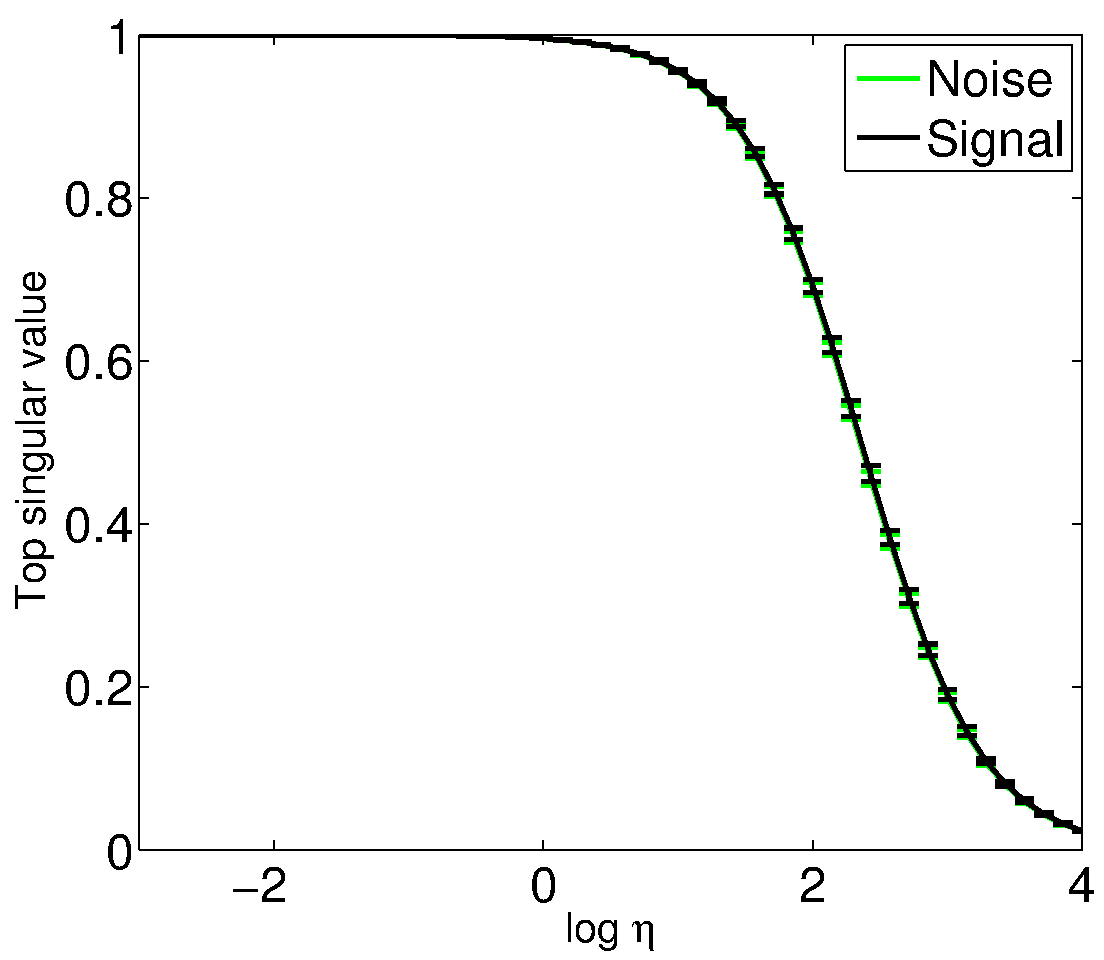
\includegraphics[width=\figwidth]{figures/rcca_errorbars_low_snr_n_50.pdf} 
} 
\subfigure[$n=150$]{
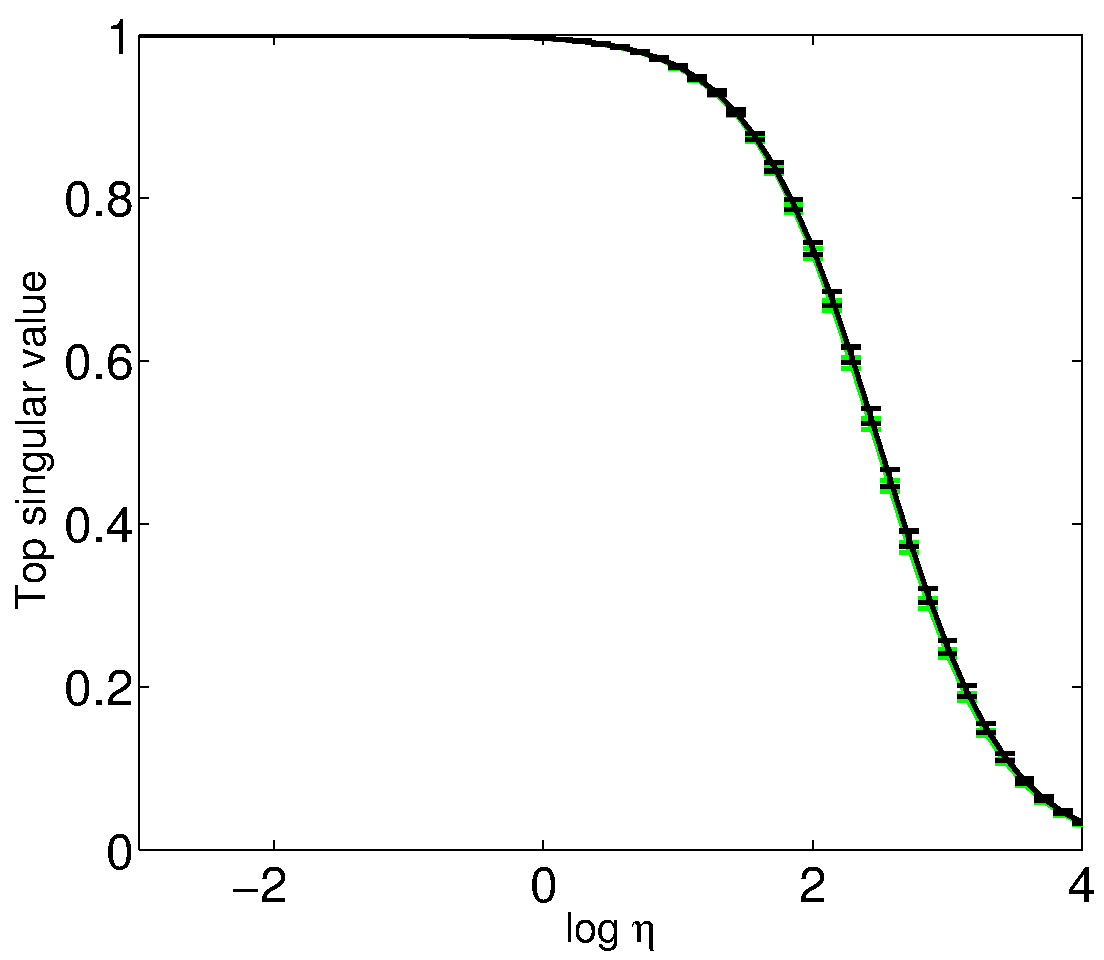
\includegraphics[width=\figwidth]{figures/rcca_errorbars_low_snr_n_150.pdf} 
} 
\subfigure[$n=300$]{
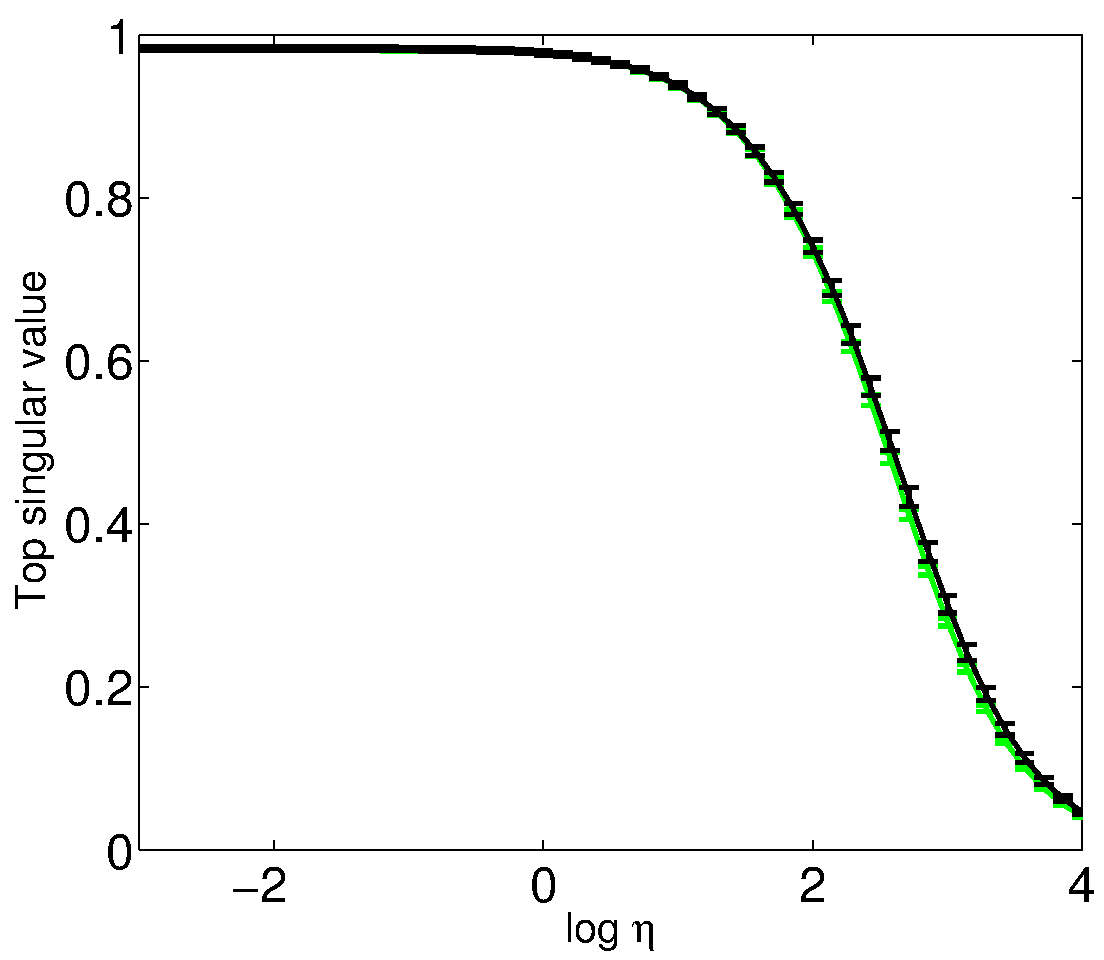
\includegraphics[width=\figwidth]{figures/rcca_errorbars_low_snr_n_300.pdf} 
} 
\subfigure[$n=600$]{
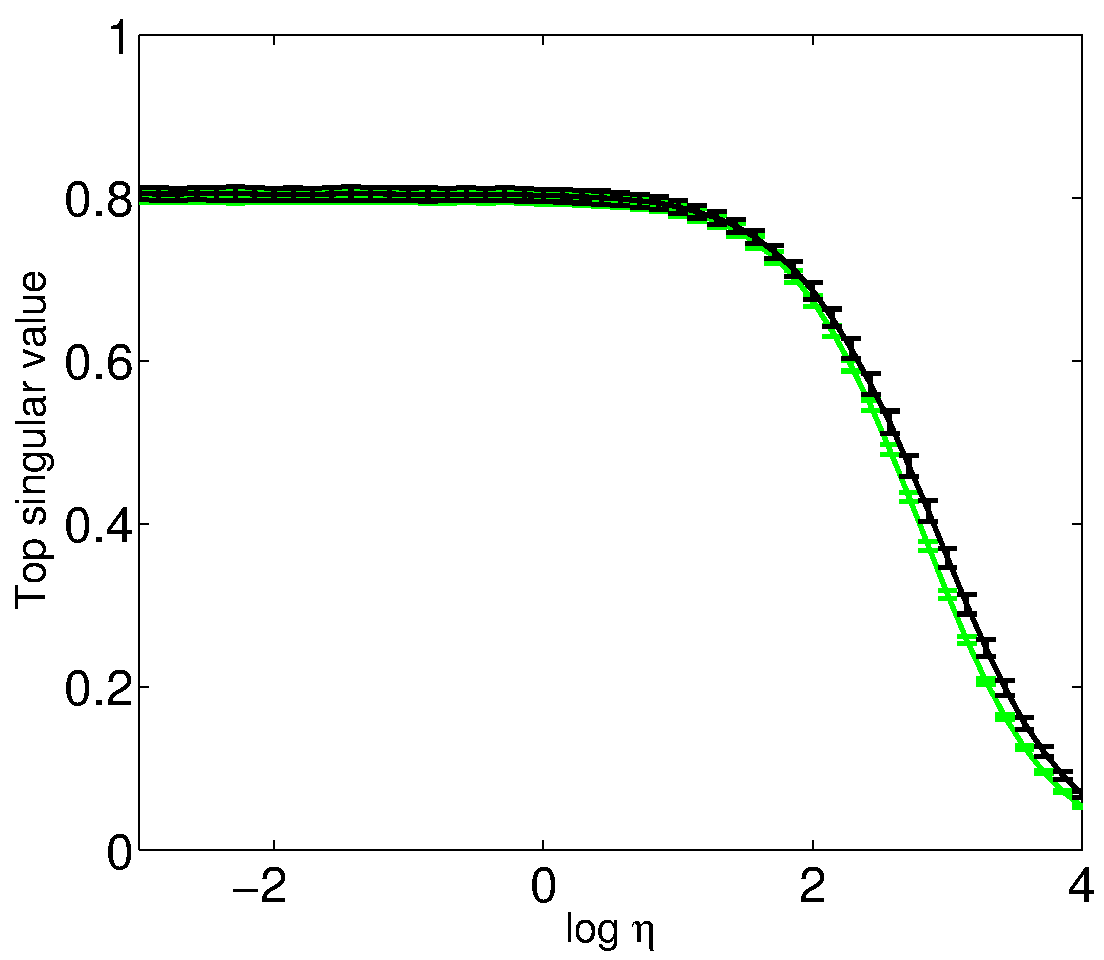
\includegraphics[width=\figwidth]{figures/rcca_errorbars_low_snr_n_600.pdf} 
} 
\caption{Empirical distribution of the top singular value of $\Creghat$ in
  (\ref{eq:creghat}) for both noise and signal data models in
  (\ref{eq:rcca_data_model1}). Simulations were conducted using $d_1=200$, $d_2=150$,
  $\rho=0.9$, and $\sigma=0$ dB. Results are shown for four values of $n$. The top
  singular value was computed for 500 trials. The mean top singular value is plotted with
  $\pm$ one standard deviation errorbars. The distribution of the top singular value of the
  noise distribution is plotted in green and that of the signal distribution is plotted in
  black.}
\label{fig:rcca_errorbars_low_snr}
\end{figure}

\begin{figure}[h!]
\subfigure[$n=50$]{
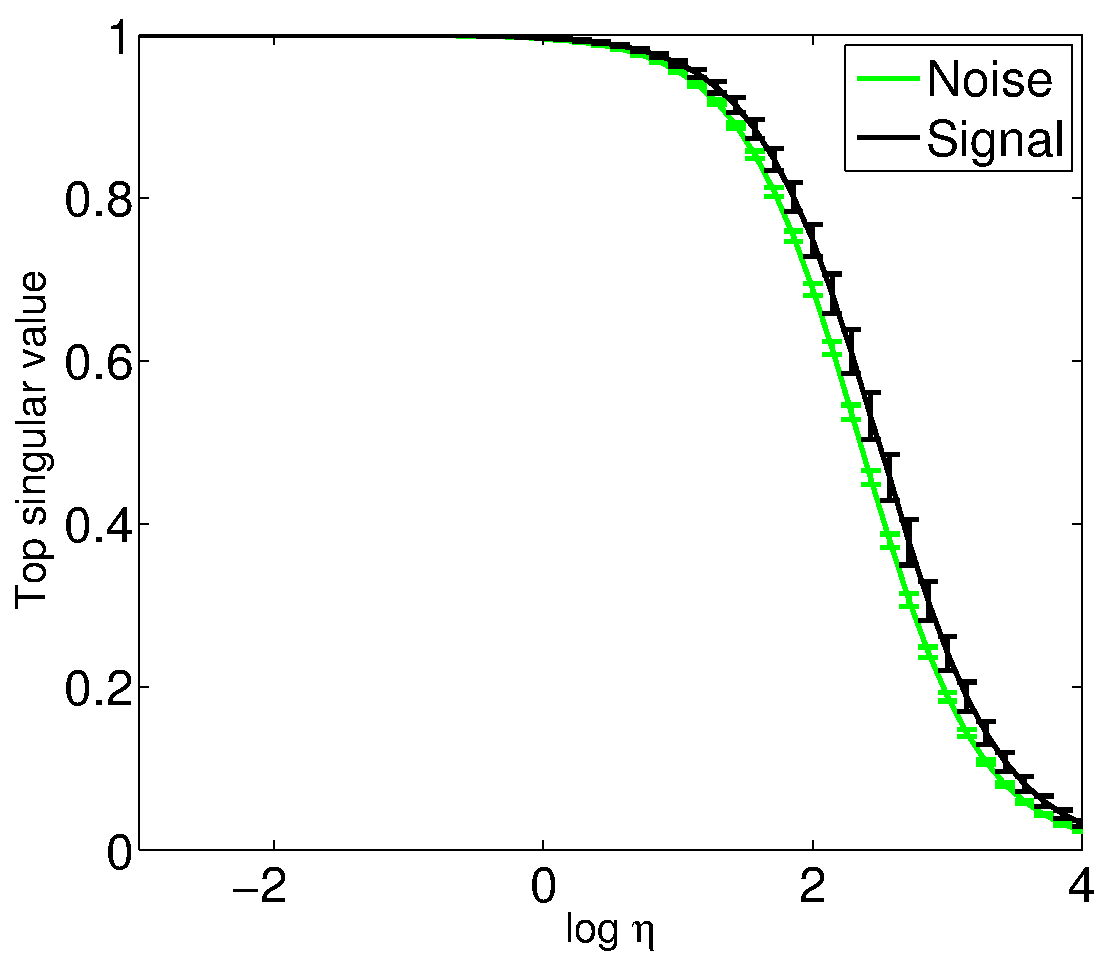
\includegraphics[width=\figwidth]{figures/rcca_errorbars_high_snr_n_50.pdf} 
} 
\subfigure[$n=150$]{
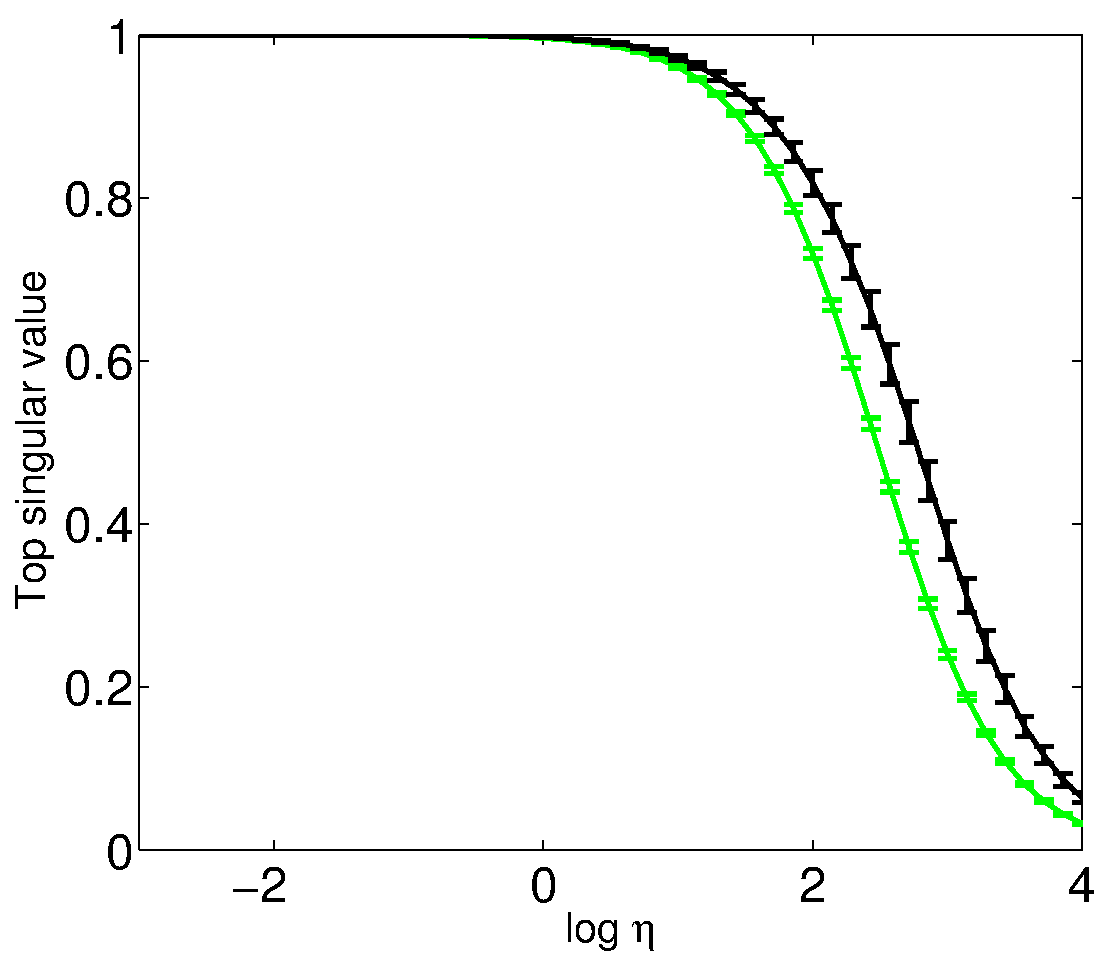
\includegraphics[width=\figwidth]{figures/rcca_errorbars_high_snr_n_150.pdf} 
} 
\subfigure[$n=300$]{
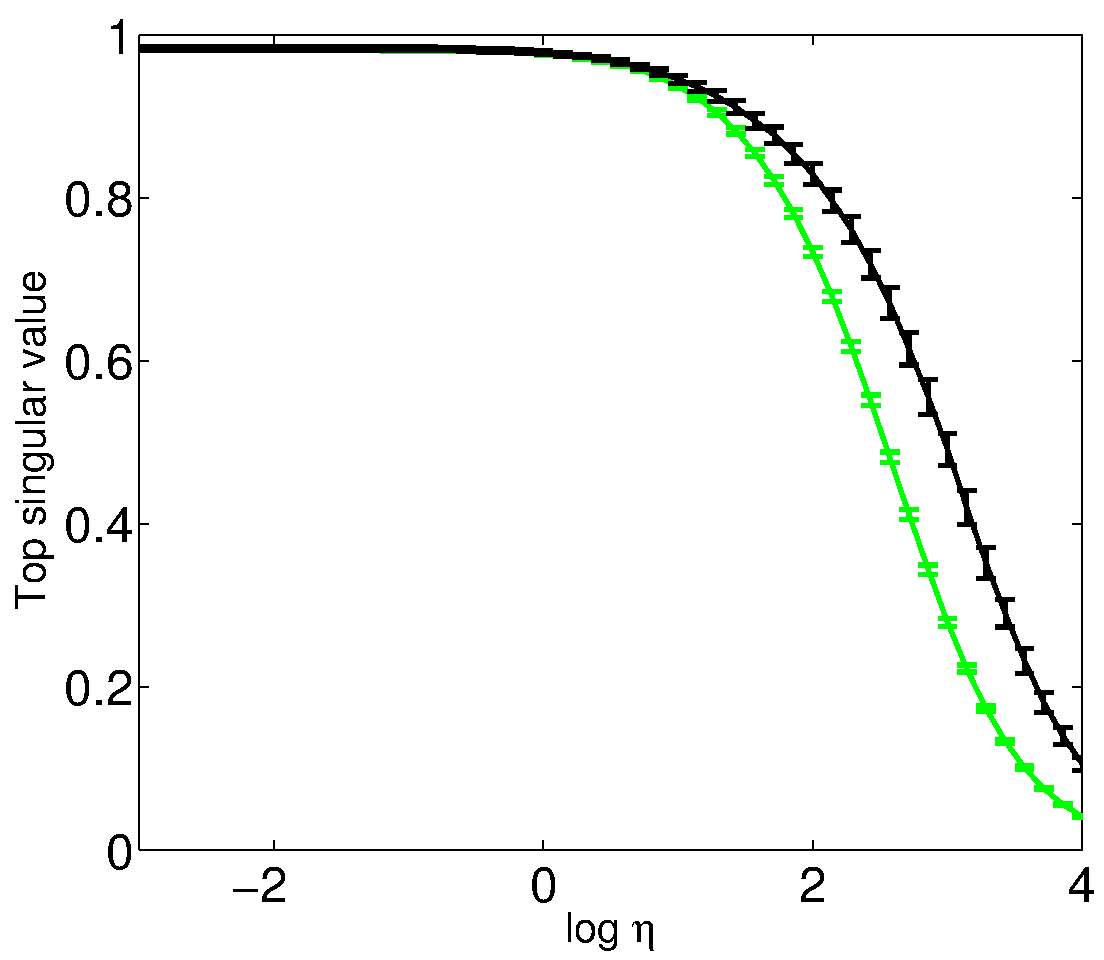
\includegraphics[width=\figwidth]{figures/rcca_errorbars_high_snr_n_300.pdf} 
} 
\subfigure[$n=600$]{
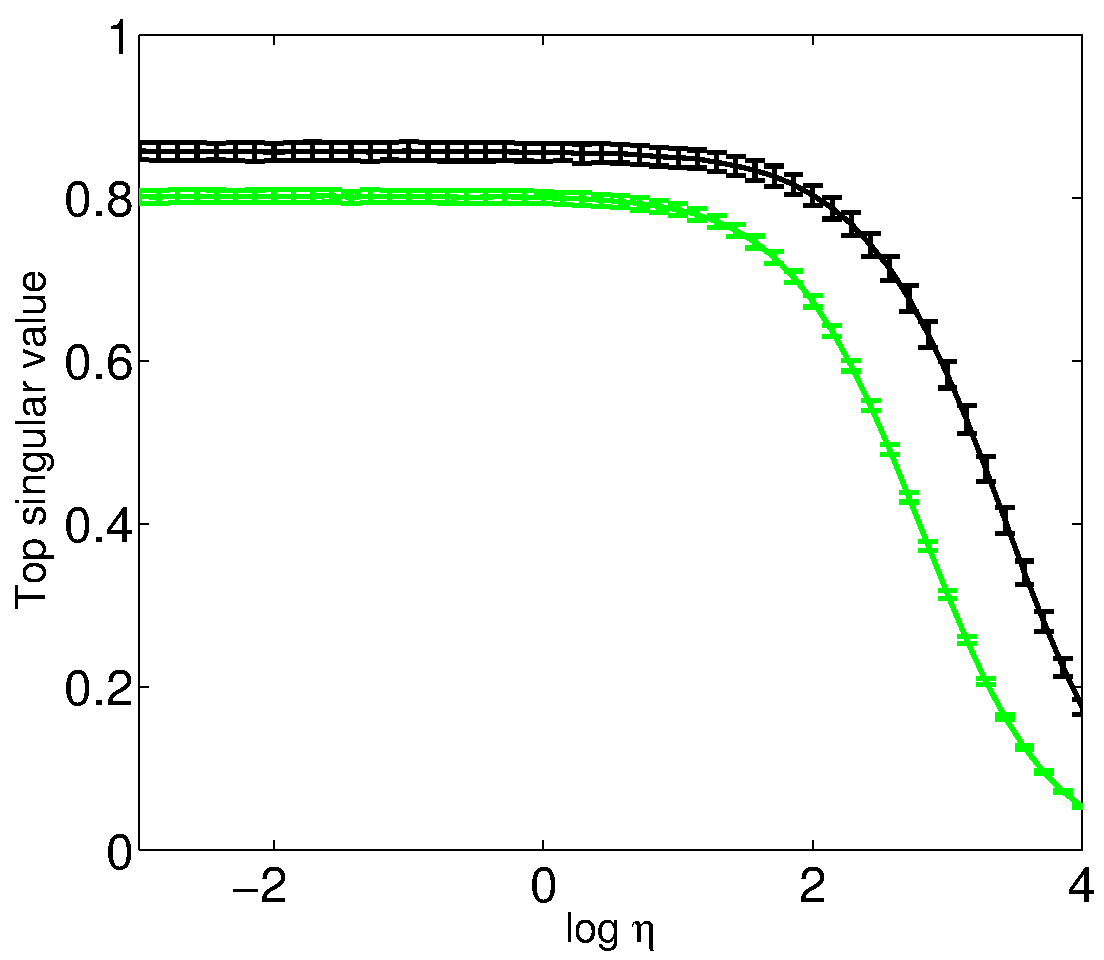
\includegraphics[width=\figwidth]{figures/rcca_errorbars_high_snr_n_600.pdf} 
} 
\caption{Empirical distribution of the top singular value of $\Creghat$ in
  (\ref{eq:creghat}) for both noise and signal data models in
  (\ref{eq:rcca_data_model1}). Simulations were conducted using $d_1=200$, $d_2=150$,
  $\rho=0.9$, and $\sigma=3$ dB. Results are shown for four values of $n$. The top singular
  value was computed for 500 trials. The mean top singular value is plotted with $\pm$ one
  standard deviation errorbars. The distribution of the top singular value of the noise
  distribution is plotted in green and that of the signal distribution is plotted in
  black.}
\label{fig:rcca_errorbars_high_snr}
\end{figure}

These figures present a number of interesting results. First, we see that for each value
of $n$, when $\eta$ is small, the value of $\widehat{\rho}$ is large under both the signal
and noise distribution. It is undesirable for $\widehat{\rho}$ to be large under the noise
distribution as this indicates a strong correlation between the datasets while in fact,
there is no correlation. 

As is expected, the noise and signal empirical distributions separate more at a larger
SNR. This is more evident at larger value of $n$. This behavior is very intuitive as one
would hope that more samples and a larger SNR would yield statistically different
distributions. A visual inspection of the distributions show that when $\sigma=3$ dB, the
distributions are completely separable when $n=600$. In fact, for all value of $n$, it
appears that the distributions separate more for larger value of $\eta$. 

When $\eta$ is increased, the value of $\widehat{\rho}$ decreases rapidly. In all eight
figures, there seems to be a phase transition in $\eta$. For low value of $\eta$,
$\widehat{\rho}$ remains relatively constant. For values of $\eta$ above a critical value,
the value of $\widehat{\rho}$ begins to decrease rapidly. Since $\eta$ controls the
magnitude of the canonical vectors, larger $\eta$ will force the canonical vectors to have
a small norm. In this regime of large $\eta$, it is possible that we are sacrificing the
accuracy of the canonical vectors to achieve better separability between the empirical
distributions of $\widehat{\rho}$. More experiments investigating the behavior of the
singular vectors are most certainly necessary. 

\subsection{Detection Based on $\widehat{\rho}$}

We next explore how well the noise and signal empirical distributions of $\widehat{\rho}$
separate. Similar to the CCA analysis, we consider the \naive detector that thresholds
based on $\rho$ to detect signal versus noise given two possibly correlated datasets. Given
the two empirical distributions for the noise and signal datasets, we construct an
empirical ROC curve. We measure the detection power of such a detector by computing the
area under the empirical ROC curve (AUC) as was done in the analysis of CCA. Figure
\ref{fig:rcca_auc_heatmap} plots the empirical AUC for such a detector for four different
values of $n$ while sweeping over both $\sigma$ and $\eta$.

\begin{figure}[h!]
\subfigure[$n=50$]{
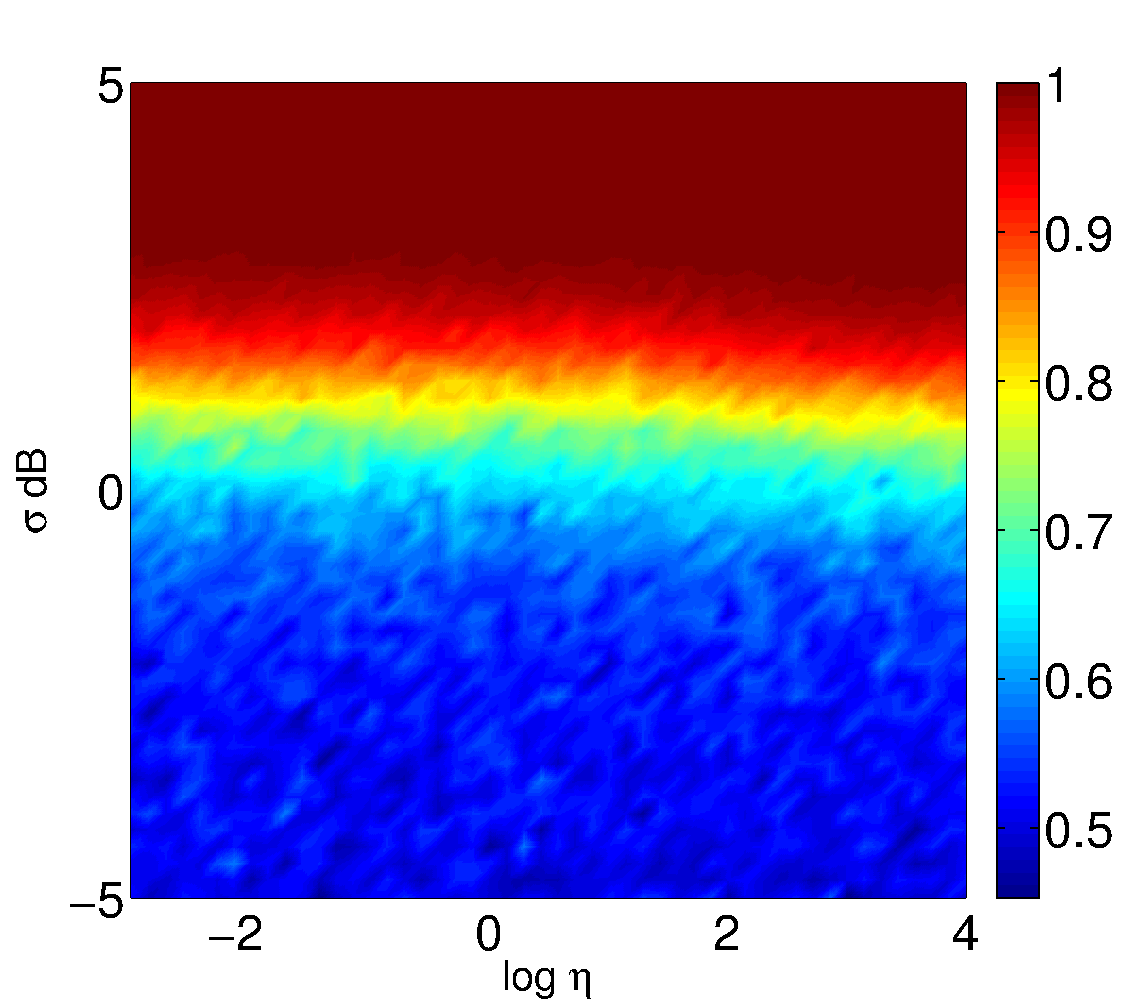
\includegraphics[width=\figwidth]{figures/rcca_auc_heatmap_n_50.pdf} 
} 
\subfigure[$n=150$]{
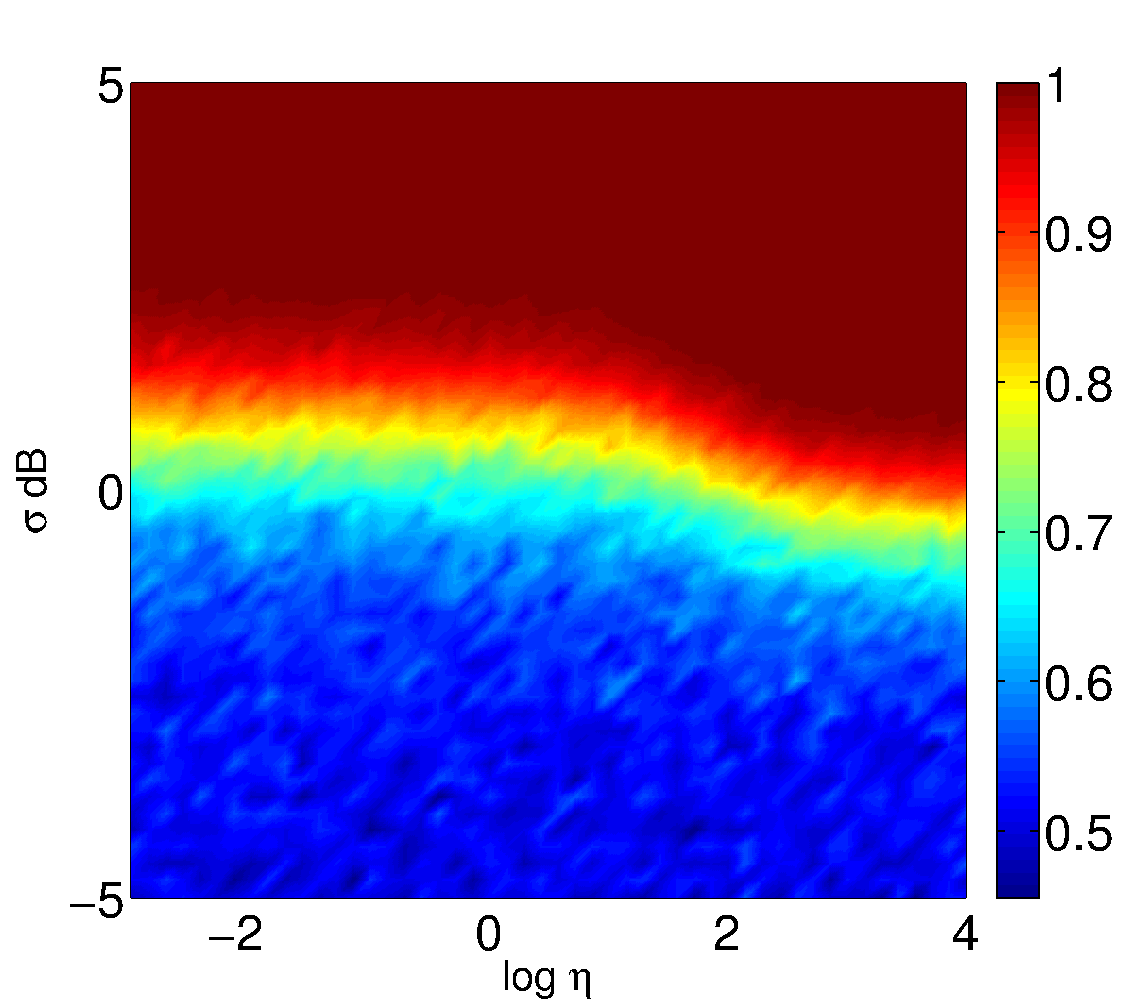
\includegraphics[width=\figwidth]{figures/rcca_auc_heatmap_n_150.pdf} 
} 
\subfigure[$n=300$]{
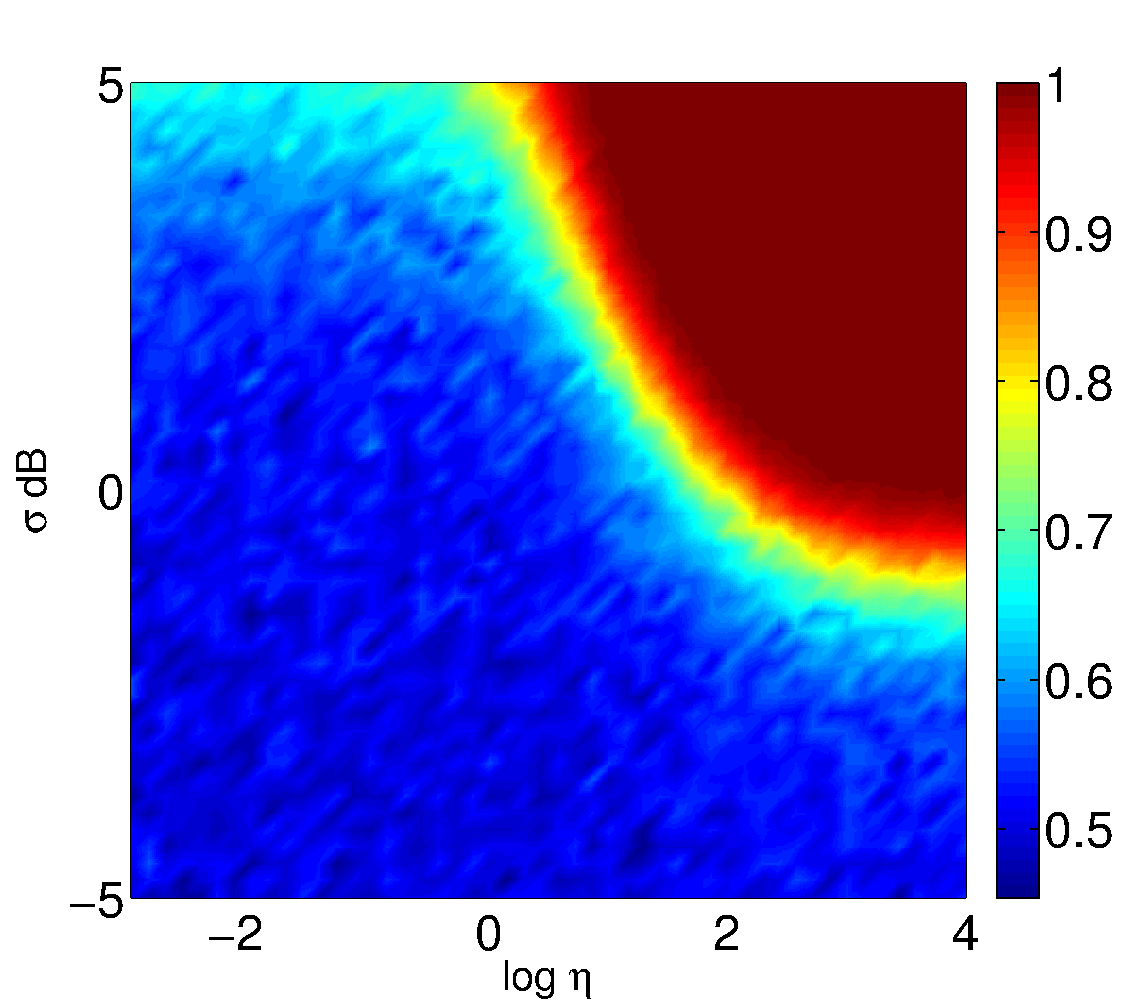
\includegraphics[width=\figwidth]{figures/rcca_auc_heatmap_n_300.pdf} 
} 
\subfigure[$n=600$]{
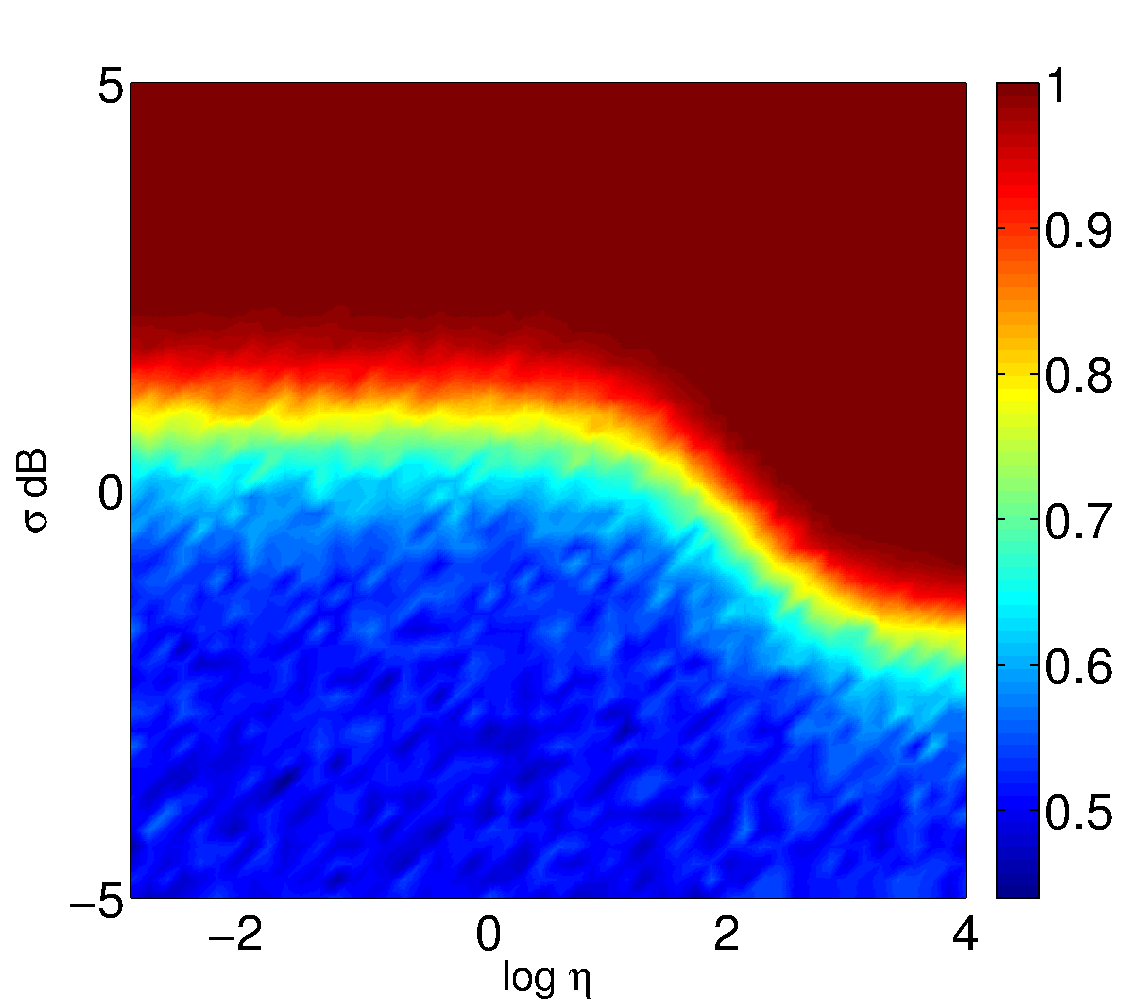
\includegraphics[width=\figwidth]{figures/rcca_auc_heatmap_n_600.pdf} 
} 
\caption{Empirical AUC of the detector based on the top singular value of $\Creghat$ in
  (\ref{eq:creghat}) based on the data models in (\ref{eq:rcca_data_model1}). Simulations
  were conducted using $d_1=200$, $d_2=150$, $\rho=0.9$, and 500 trials. Results are
  shown for 4 values of $n$. In each figure, the AUC is plotted for multiple combinations
  of $\sigma$ and $\eta$.}
\label{fig:rcca_auc_heatmap}
\end{figure}

First we see that in the sample poor regime when $n=50$, RCCA allows detection of the
target signal. Compared to Figure \ref{fig:cca_auc_heatmap}, RCCA drastically increases
detection ability in this low sample regime. There is a critical value of SNR under which
the target signal may no longer be reliably detected. The performance of such a detector
in this sample poor regime seems to be unaffected by the choice of regularization
parameter.

When increasing the number of samples to $n=150$, we see an interesting phenomena. With
more samples, we seem to be able to tolerate a slightly lower value of $\sigma$ to achieve
the same performance as the detector using $n=50$ training samples. This is intuitive and
desirable. We are still operating in the regime of $n<d_1+d_2$ where CCA breaks
down. However, RCCA is now able to reliably detect the presence of signal. The phenomena
arises when considering the affect of $\eta$. We see that if we allow $\eta$ to be very
large, we can increase in the detection ability of the \naive detector based on
$\widehat{k}_1$. Again, we may be sacrificing the accuracy of the canonical vectors to
gain this increased detection ability.

An extremely interesting phenomena arises when increasing $n$ to 300. In this regime, we
are still have $n<d_1+d_2$ but we have enough samples that $\RIhat$ and $\RIIhat$ are both
full rank. We now see a large portion of the heatmap indicate that the detector has no
detection ability. Unlike the detectors using less samples, this detector must have a
large enough regularization parameter to have useful detection ability. Similar to the
detector using $n=150$ samples, if we allow $\eta$ to increase large enough, we can
tolerate a much smaller SNR and still achieve good detection ability. The behavior of RCCA
seems to be highly dependent on both the number of samples and the value of the
regularization parameter. This is very undesirable.

Finally, when we increase $n$ to 600, we return to a similar behavior when $n=150$. For
lower values of $\eta$, we seem to have approximately the same performance as the
detectors using $n=50$ and $n=150$ samples. This is very undesirable as the more training
samples that we have, the better performance we should achieve. Again we see that by
increasing $\eta$ large enough, we can tolerate a much smaller SNR to achieve the same AUC
performance. Future work describing how the regularization parameter affects the canonical
vectors is of utmost importance.

\section{Informative RCCA (IRCCA)}

In this section, we apply the ideas of informative CCA to regularized CCA. As seen in the
previous section, the performance of RCCA is irregular and highly dependent on the choice
of the regularization parameter and number of samples. We first derive an informative
version of RCCA (IRCCA) and show, through numerical simulations, that it has a more
consistent performance that is not dependent on the regularization parameter and which
improves with more training samples. We compare the performance of RCCA and IRCCA when
used for signal detection and highlight parameter regimes where each works best.

\subsection{IRCCA Derivation}

We begin by recalling the singular value decompositions of the data matrices, $Y_1 =
U_1\Sigma_1V_1^H$ and $Y_2= U_2\Sigma_2V_2$.  Examining (\ref{eq:rcca_chat_decomp}), we
observe that the estimate for the maximum correlation between the datasets is
\begin{equation}\label{eq:rcca_rhohat}
\widehat{\rho} = \sigma_1(\Creghat) = \sigma_1\left((\Sigma_1\Sigma_1^H+\eta
I_{d_1})^{-1/2}\Sigma_1V_1^HV_2\Sigma_2^H(\Sigma_2\Sigma_2^H + \eta
I_{d_2})^{-1/2}\right).
\end{equation}
From this expression, it is clear that RCCA relies on the matrix product $V_1^HV_2$. This
term most likely causes the irregularity in the performance of RCCA as it broke the
performance of CCA in the sample starved regime. Following the guidance in Proposition
\ref{prop:raj}, we only want to use the singular vectors of $V_1$ and $V_2$ that are
informative. In low-rank systems, this proposition tells us that many of these right
singular vectors are uninformative and using them would only introduce additional noise
into the algorithm. Following the approach in CCA, we define the trimmed data matrices
\be\ba
&\widetilde{\Sigma}_1=\Sigma_1(1:r_1,1:r_1) &&\widetilde{\Sigma}_2=\Sigma_2(1:r_2,1:r_2)\\
&\widetilde{U}_1=U_1(:,1:r_1) &&\widetilde{U}_2=U_2(:,1:r_2)\\
&\widetilde{V}_1=V_1(:,1:r_1) &&\widetilde{V}_2=V_2(:,1:r_2)\\
\ea\ee where $r_1$ and $r_2$ are the number of informative components computed by
Proposition \ref{prop:raj} in the first and second datasets, respectively.

Using these trimmed data matrices results in an informative RCCA (IRCCA) algorithm. We
first construct
\beq\label{eq:cregtil}
\Cregtil = \widetilde{U}_1(\widetilde{\Sigma}_1\widetilde{\Sigma}_1^H+ \eta
I_{r_1})^{-1/2}\widetilde{\Sigma}_1\widetilde{V}_1^H\widetilde{V}_2\widetilde{\Sigma}_2^H
(\widetilde{\Sigma}_2\widetilde{\Sigma}_2^H + \eta I_{r_2})^{-1/2}\widetilde{U}_2^H 
\eeq
and then take the SVD $\Cregtil = \widetilde{F}\widetilde{K}\widetilde{G}^H$. The IRCCA
canonical vectors and correlation coefficient estimates are
\be\ba
& \widetilde{\rho} = \widetilde{k}_1\\
& \widetilde{x}_1 = (\RIhat+\eta I_{d_1})^{-1/2}\widetilde{f}_1\\
& \widetilde{x}_2 = (\RIIhat+\eta I_{d_2})^{-1/2}\widetilde{g}_1.\\
\ea\ee

\subsection{Numerical Simulations}

We use the same simulation setup as in RCCA above, generating $n$ samples from
(\ref{eq:rcca_data_model1}) to form $Y_1^{\text{noise}}$, $Y_2^{\text{noise}}$,
$Y_1^{\text{signal}}$, and $Y_2^{\text{signal}}$. We use these training data matrices to
compute $\Cregtil^{\text{noise}}$ and $\Cregtil^{\text{signal}}$ as in
(\ref{eq:cregtil}). For two values of $\sigma$, figures \ref{fig:rcca_errorbars_low_snr}
and \ref{fig:rcca_errorbars_high_snr} plot the empirical distributions of the IRCCA
correlation estimate, $\widetilde{\rho}$, generated from the SVD of
$\Cregtil^{\text{noise}}$ and $\Cregtil^{\text{signal}}$. The RCCA correlation estimate,
$\widehat{\rho}$, is also plotted for comparison.

\begin{figure}[h!]
\subfigure[$n=50$]{
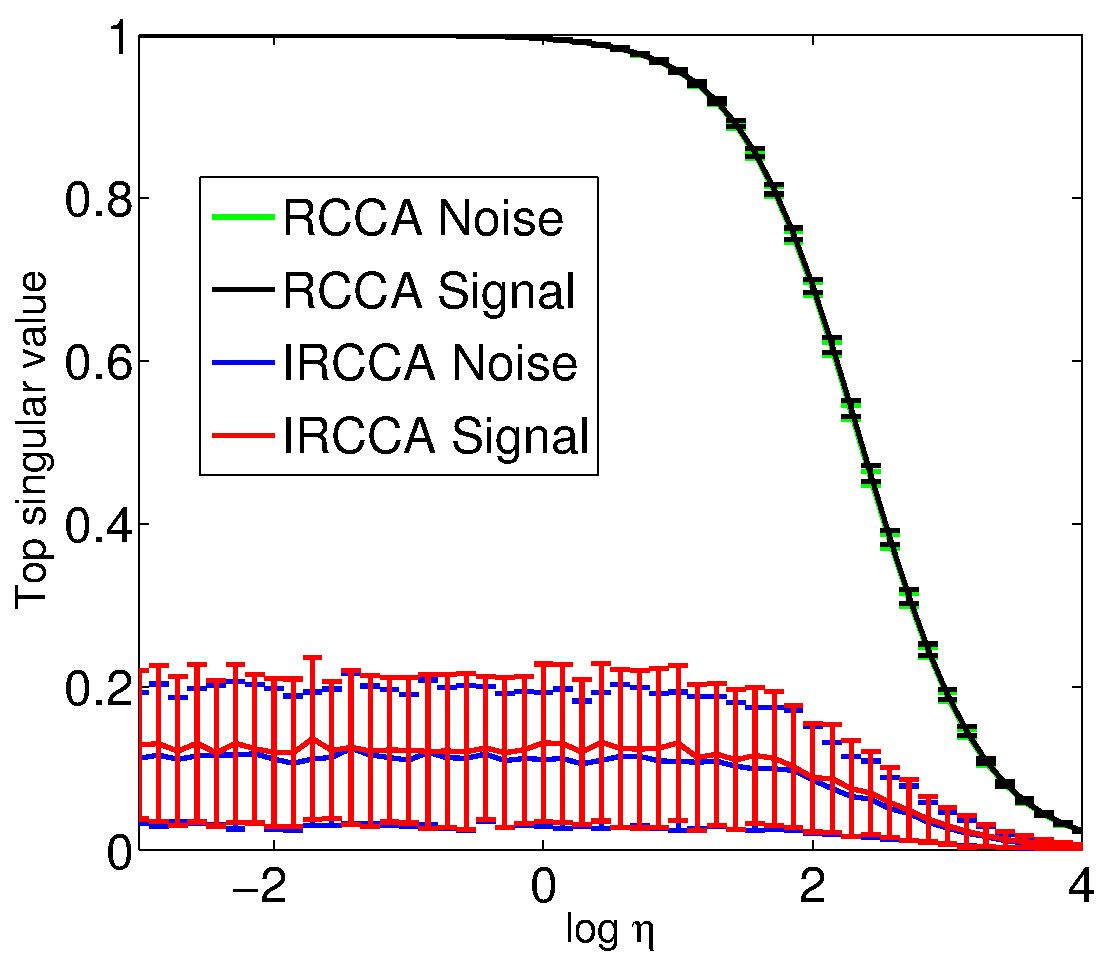
\includegraphics[width=\figwidth]{figures/ircca_errorbars_low_snr_n_50.pdf} 
} 
\subfigure[$n=150$]{
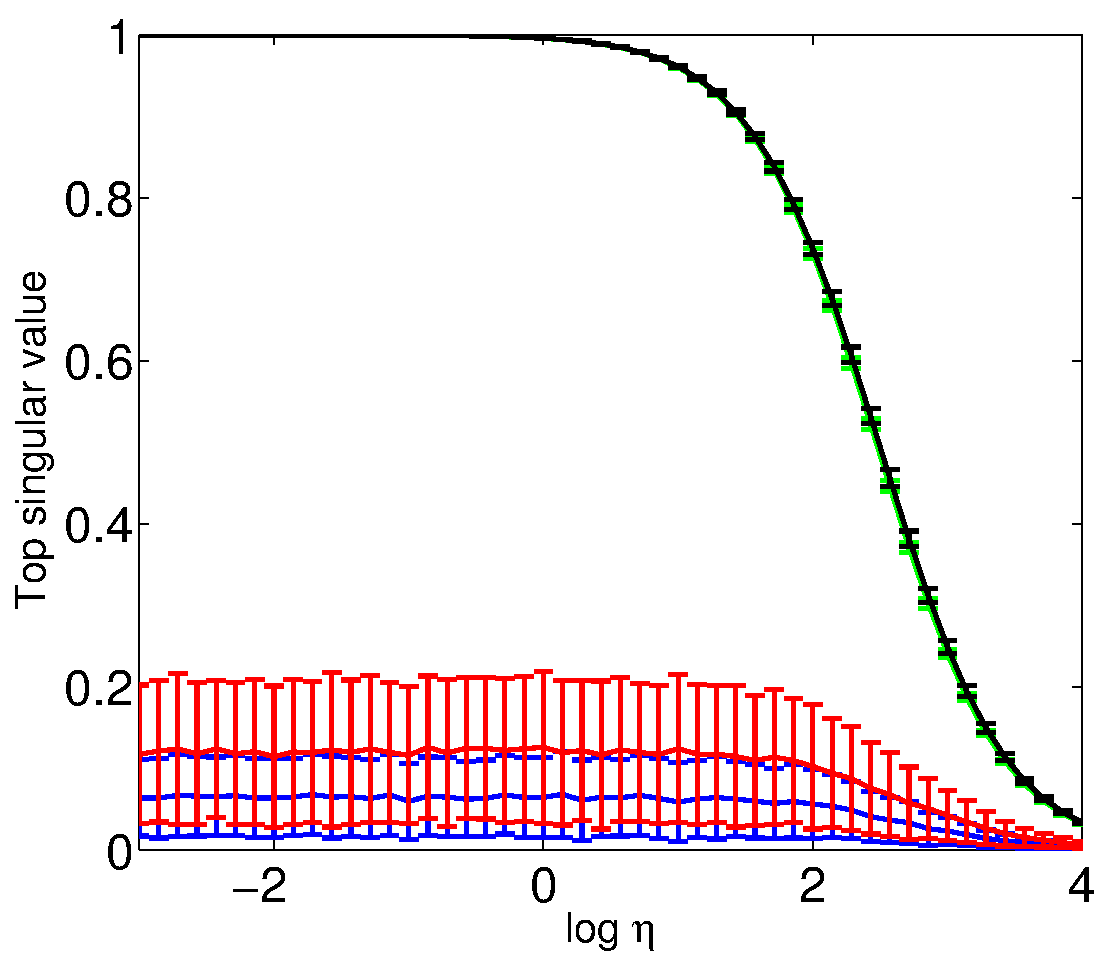
\includegraphics[width=\figwidth]{figures/ircca_errorbars_low_snr_n_150.pdf} 
} 
\subfigure[$n=300$]{
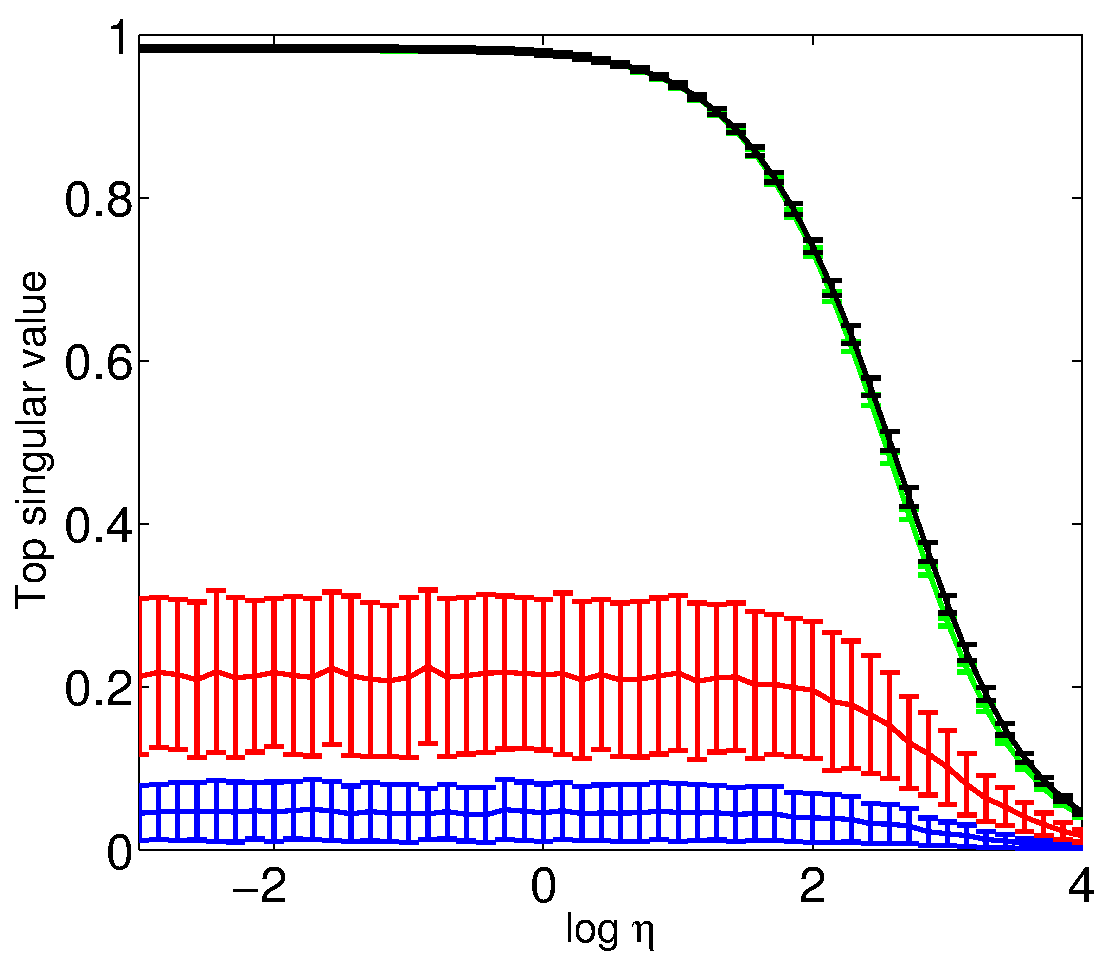
\includegraphics[width=\figwidth]{figures/ircca_errorbars_low_snr_n_300.pdf} 
} 
\subfigure[$n=600$]{
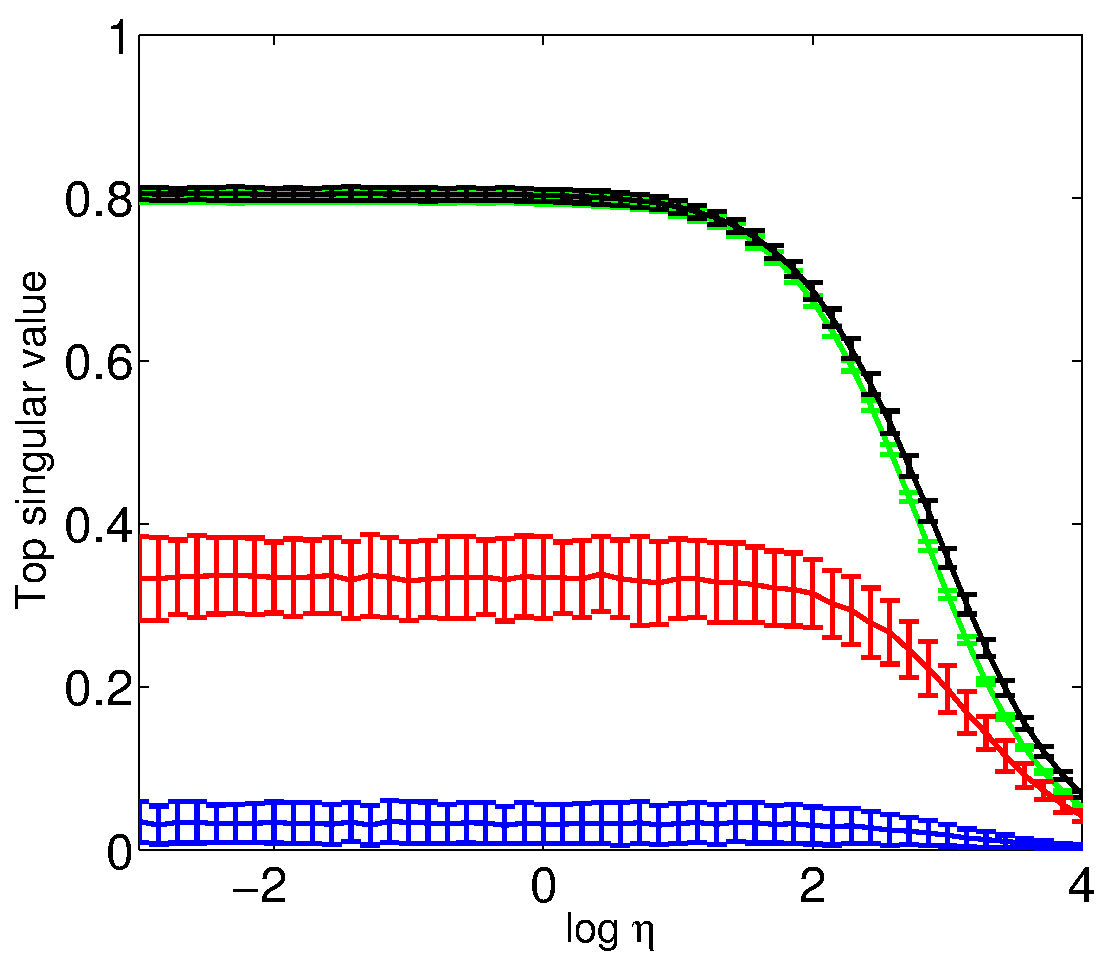
\includegraphics[width=\figwidth]{figures/ircca_errorbars_low_snr_n_600.pdf} 
} 
\caption{Empirical distribution of the top singular value of $\Cregtil$ in
  (\ref{eq:cregtil}) for both noise and signal data models in
  (\ref{eq:rcca_data_model1}). Simulations were conducted using $d_1=200$, $d_2=150$,
  $\rho=0.9$, and $\sigma=0$ dB. Results are shown for four values of $n$. The top
  singular value was computed for 500 trials. The mean top singular value is plotted with
  $\pm$ one standard deviation errorbars. The figure plots the distribution of the top
  singular value of the RCCA noise distribution (green), RCCA signal distribution (black),
  IRCCA noise distribution (blue), and IRCCA signal distribution (red).}
\label{fig:rcca_errorbars_low_snr}
\end{figure}

\begin{figure}[h!]
\subfigure[$n=50$]{
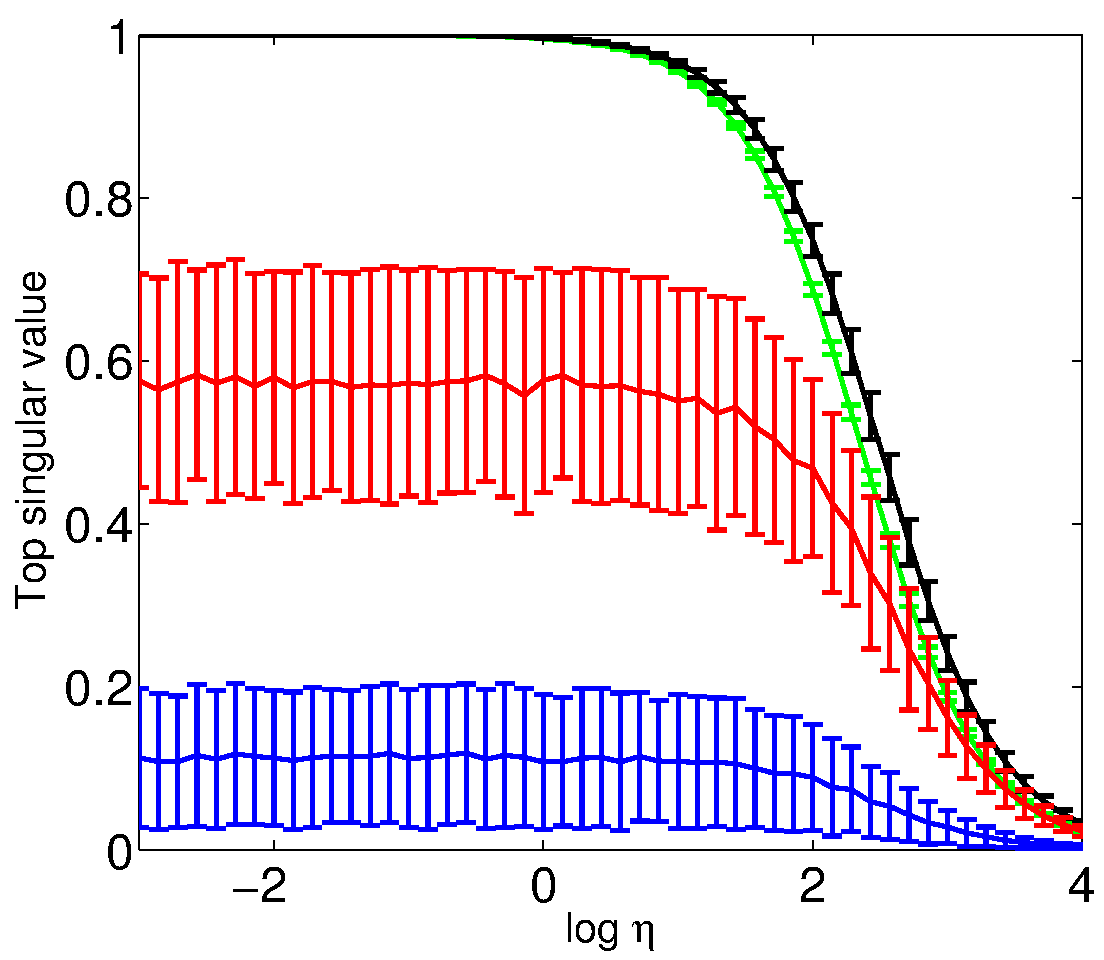
\includegraphics[width=\figwidth]{figures/ircca_errorbars_high_snr_n_50.pdf} 
} 
\subfigure[$n=150$]{
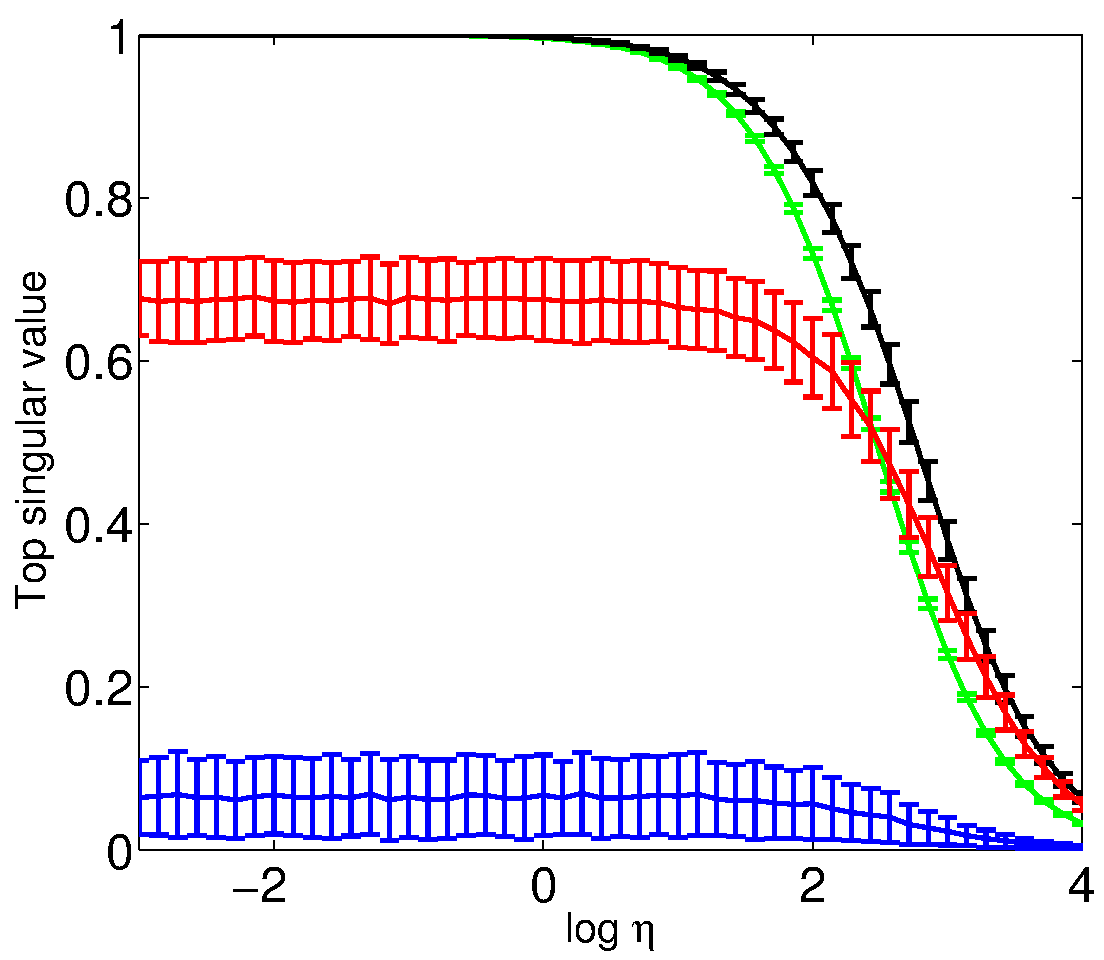
\includegraphics[width=\figwidth]{figures/ircca_errorbars_high_snr_n_150.pdf} 
} 
\subfigure[$n=300$]{
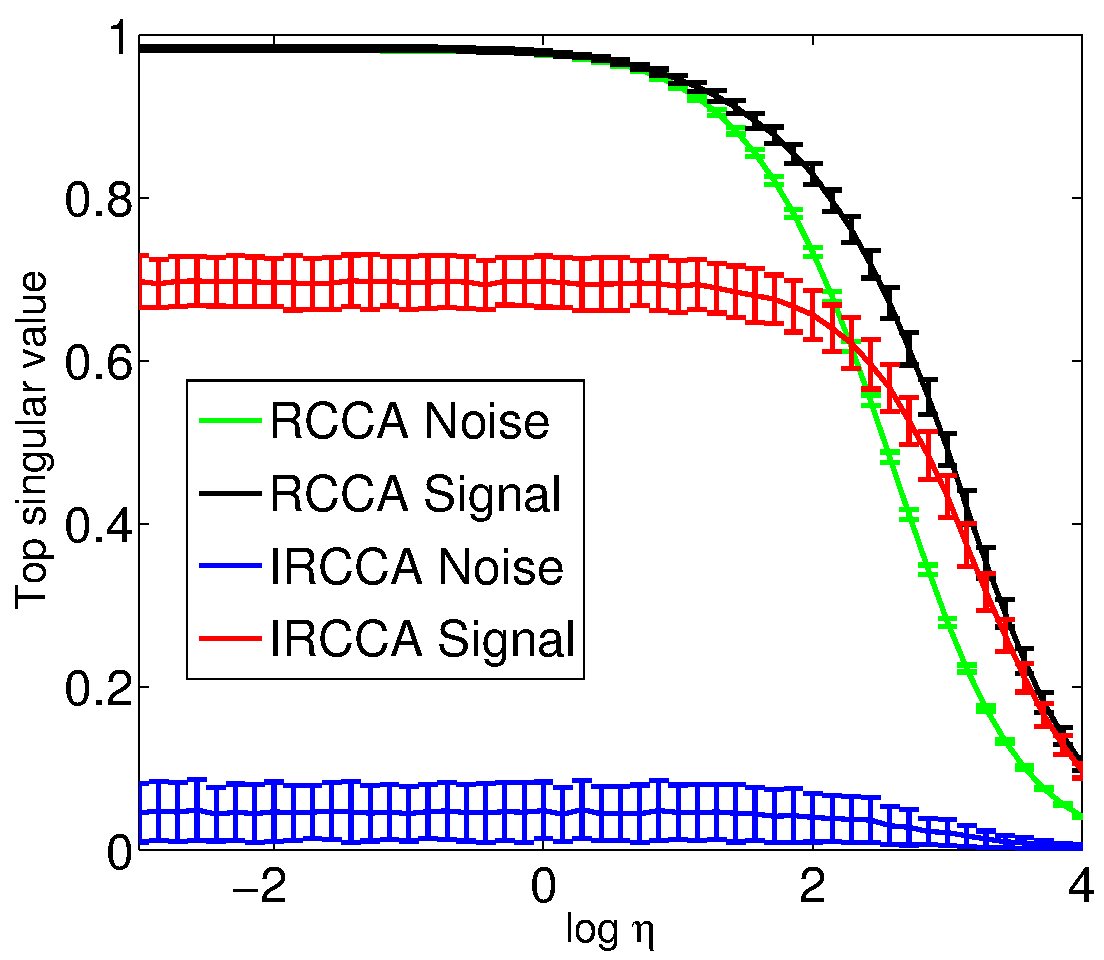
\includegraphics[width=\figwidth]{figures/ircca_errorbars_high_snr_n_300.pdf} 
} 
\subfigure[$n=600$]{
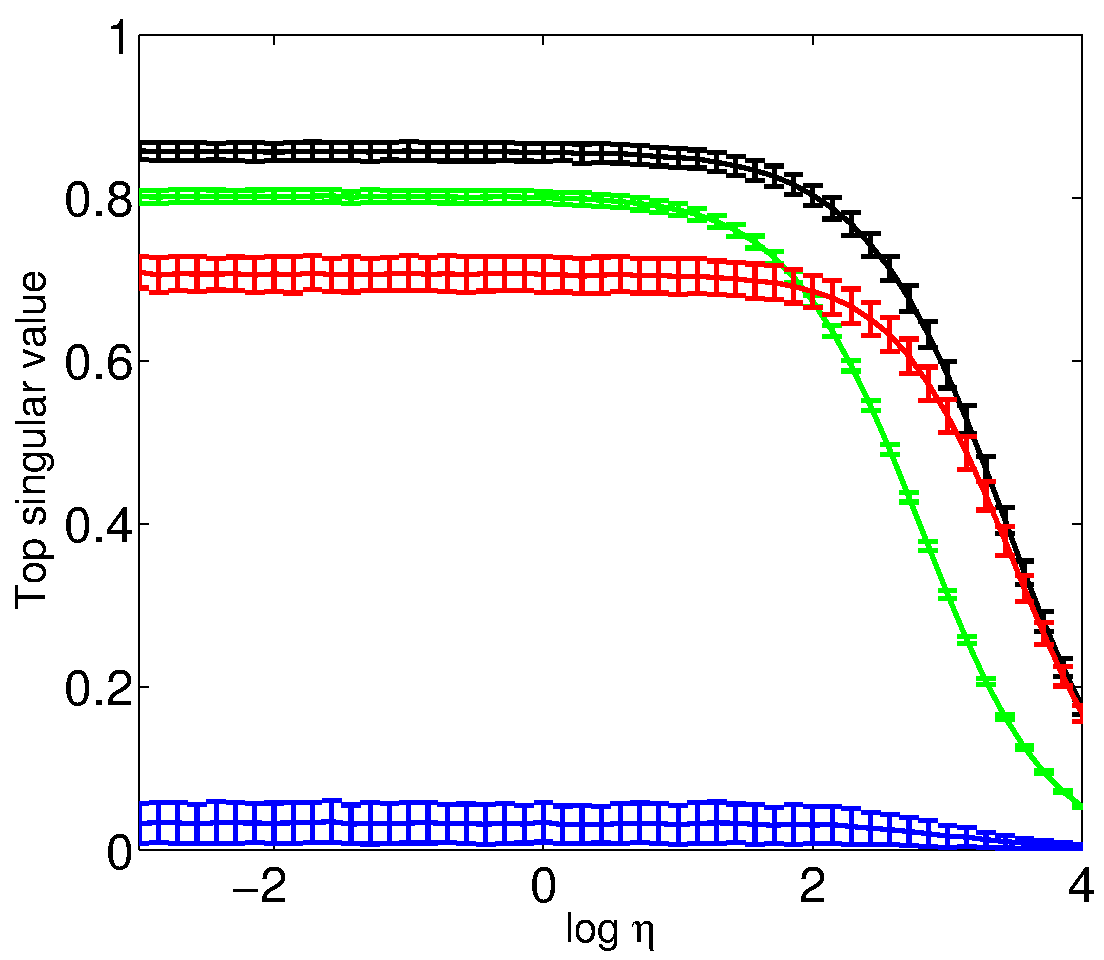
\includegraphics[width=\figwidth]{figures/ircca_errorbars_high_snr_n_600.pdf} 
} 
\caption{Empirical distribution of the top singular value of $\Creghat$ in
  (\ref{eq:creghat}) for both noise and signal data models in
  (\ref{eq:rcca_data_model1}). Simulations were conducted using $d_1=200$, $d_2=150$,
  $\rho=0.9$, and $\sigma=3$ dB. Results are shown for four values of $n$. The top
  singular value was computed for 500 trials. The mean top singular value is plotted with
  $\pm$ one standard deviation errorbars. The figures plots the distribution of the top
  singular value of the RCCA noise distribution (green), RCCA signal distribution (black),
  IRCCA noise distribution (blue), and IRCCA signal distribution (red).}
\label{fig:rcca_errorbars_high_snr}
\end{figure}

Figures \ref{fig:rcca_errorbars_low_snr} and \ref{fig:rcca_errorbars_high_snr} demonstrate
that the correlation estimate of IRCCA has many desirable properties. First, for both
values of SNR presented, the correlation estimate of the noise distribution decreases with
increased training samples. The datasets under the noise distribution are not correlated
and so it is desirable that IRCCA returns a correlation estimate close to zero and that
IRCCA becomes more confident that there is no correlation when more training samples are
available. 

Second, for both values of SNR presented, the IRCCA correlation estimate for the signal
distribution increases with more training samples. The datasets under the signal
distribution are highly correlated ($\rho=0.9$) and so it is desirable that IRCCA becomes
more confident that there is a correlation when more training samples are available. This
estimated correlation distribution is also larger for the larger value of SNR in
Figure \ref{fig:rcca_errorbars_high_snr}. It is also very desirable that IRCCA becomes more
confident that there is correlation when the SNR of the low-rank signal becomes stronger. 

Similar to the performance of RCCA, IRCCA also seems to exhibit a phase transition in the
correlation estimate that is dependent on $\eta$. For smaller values of $\eta$, the value
of $\widetilde{\rho}$ is constant for both the signal and noise data model. However, once
$\eta$ is increased past a certain threshold, the value of $\widetilde{\rho}$ decreases
rapidly. As suggested in the discussion of the performance of RCCA, we speculate that this
is due to overfitting and that the canonical vectors may be very inaccurate. Future work
examining the accuracy of the canonical vectors of both RCCA and IRCCA is paramount for
the thesis.

Visually, IRCCA seems to do a better job at separating the noise and signal distributions
for lower values of $n$ and for lower values of $\sigma$. However, visually examining
these distributions does not give an indication of how well we can distinguish between the
two. Instead, we perform the same AUC analysis as done in the RCCA analysis, using
$\widetilde{\rho}$ as the statistic for a \naive detector. We compute the empirical ROC
curve from the empirical distributions and then compute the AUC to determine the detection
ability of the detector. Figures \ref{fig:ircca_auc_heatmap1} and
\ref{fig:ircca_auc_heatmap2} show the AUC for the IRCCA detector for many values of $\eta$
and $\sigma$. The difference plot between IRCCA and RCCA is plotted for
comparison. Positive values represent that IRCCA does better. Negative values represent
that RCCA does better.

\begin{figure}[h!]
\subfigure[IRCCA, $n=50$]{
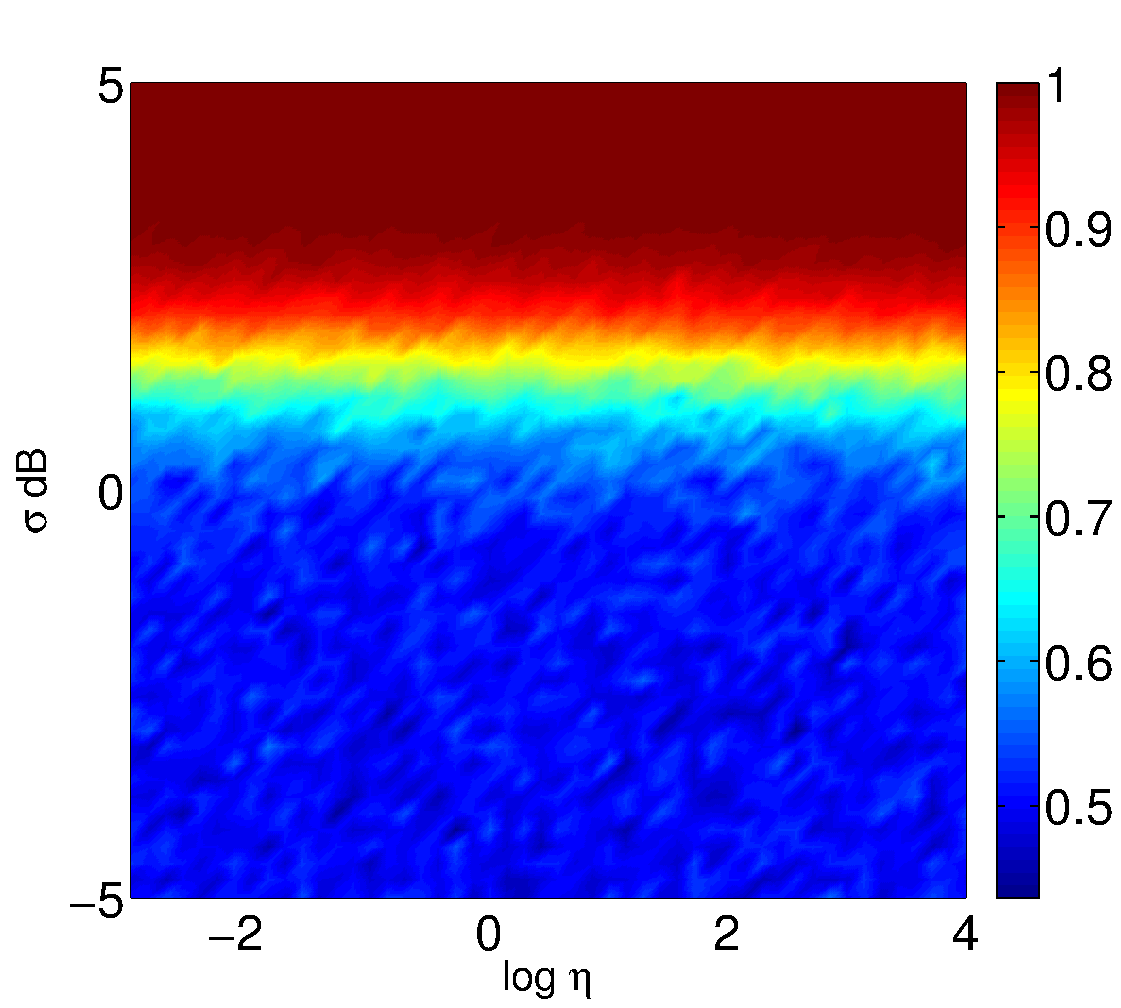
\includegraphics[width=\figwidth]{figures/ircca_auc_heatmap_n_50.pdf} 
} 
\subfigure[RCCA Difference, $n=50$]{
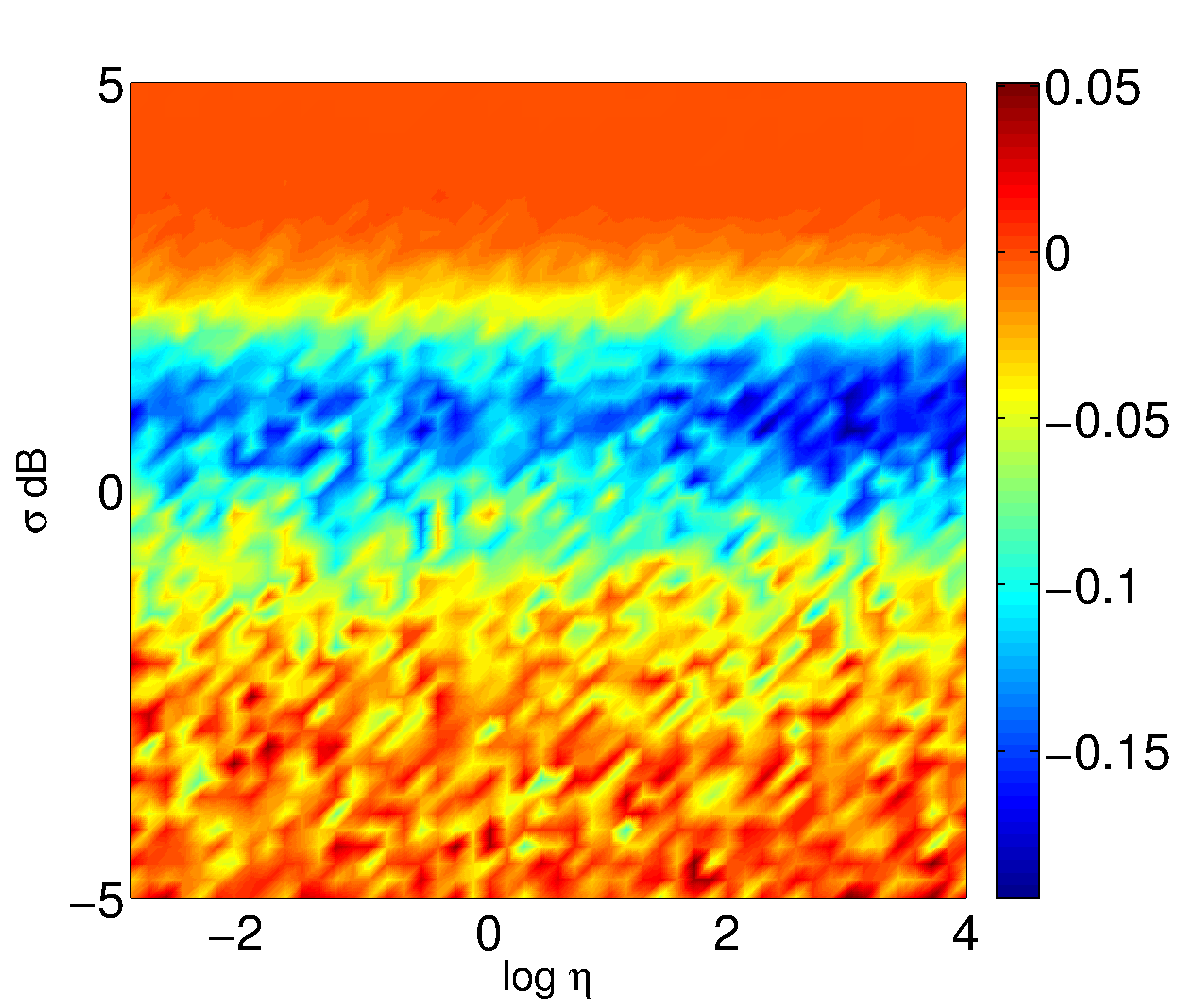
\includegraphics[width=\figwidth]{figures/ircca_auc_heatmap_diff_n_50.pdf} 
} 
\subfigure[IRCCA, $n=150$]{
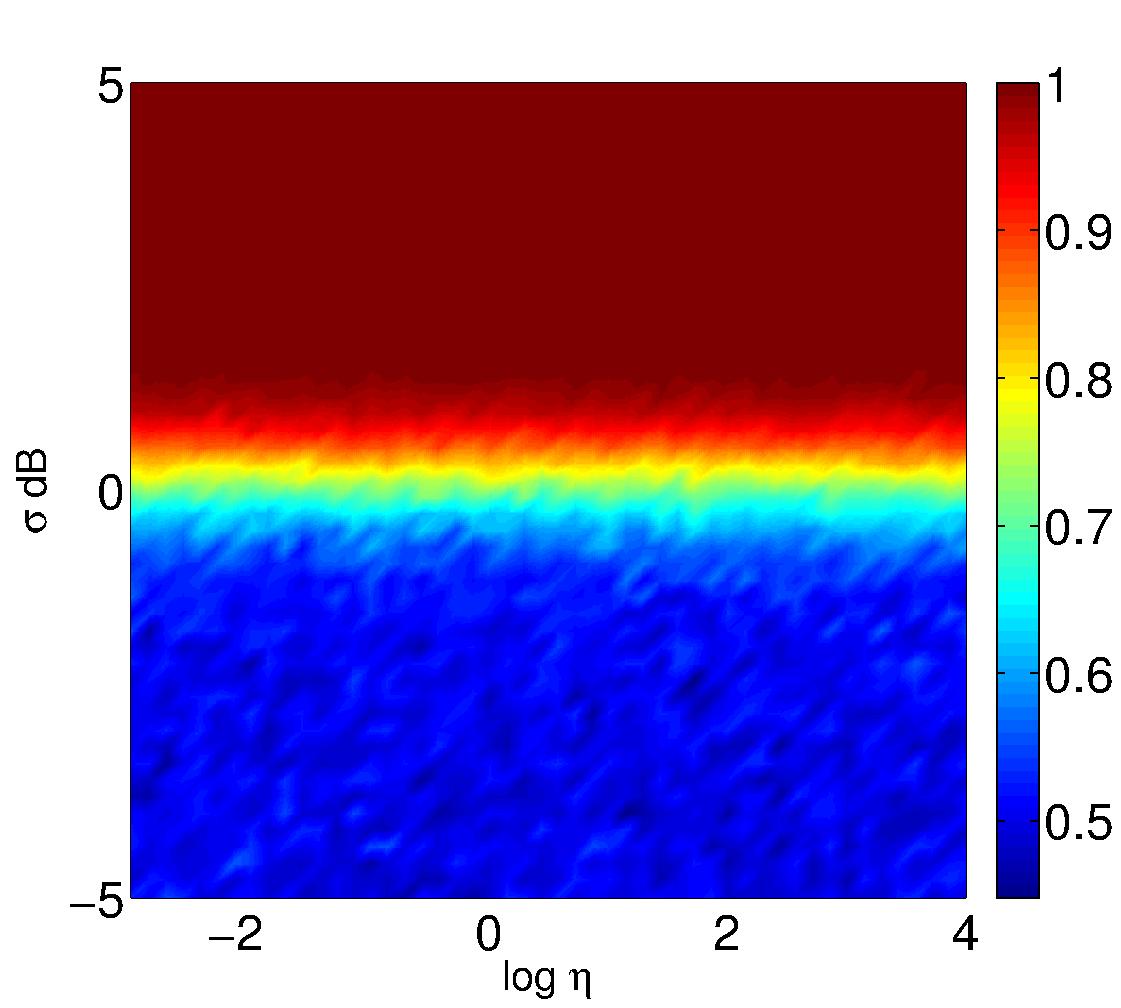
\includegraphics[width=\figwidth]{figures/ircca_auc_heatmap_n_150.pdf} 
} 
\subfigure[RCCA Difference, $n=150$]{
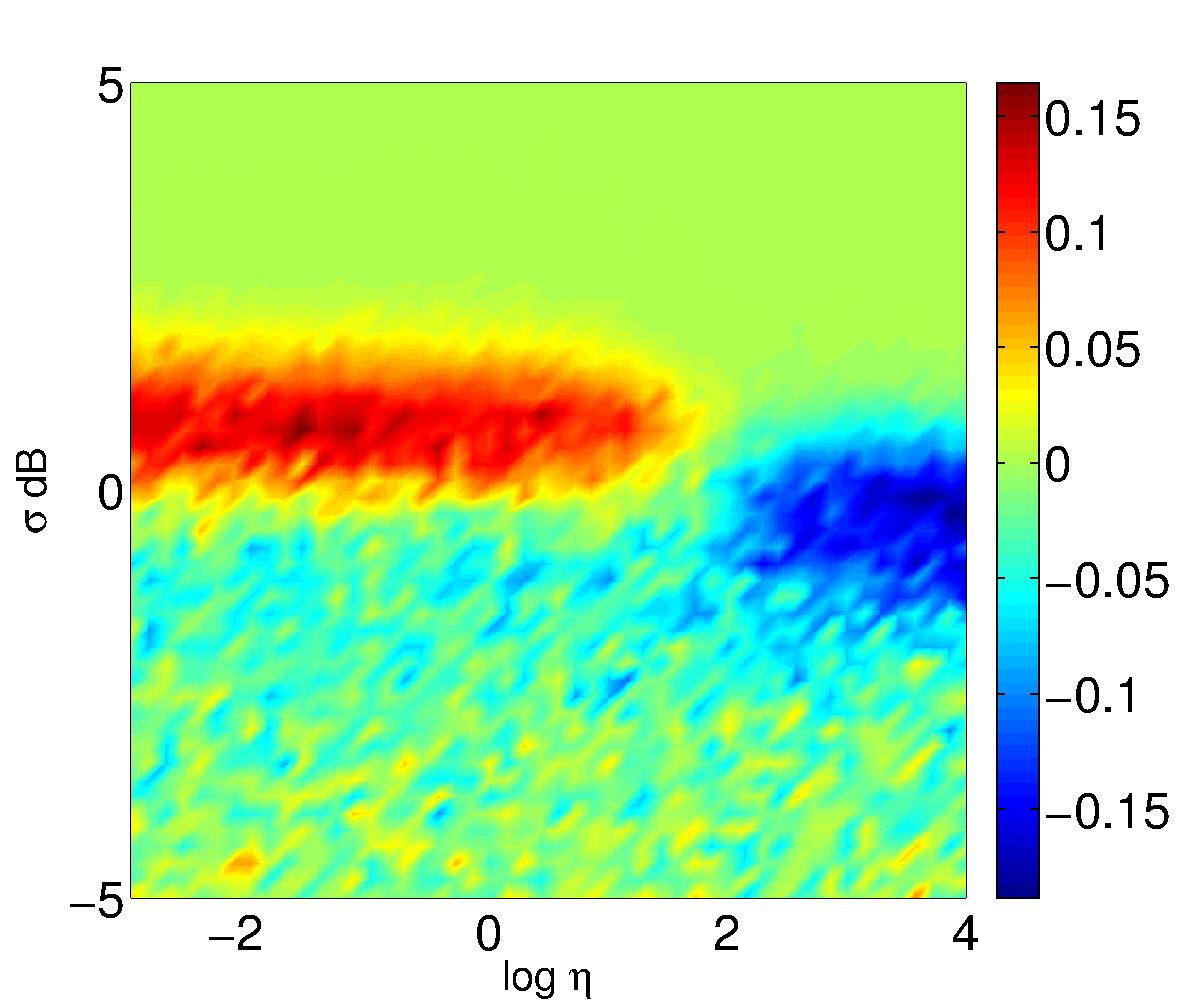
\includegraphics[width=\figwidth]{figures/ircca_auc_heatmap_diff_n_150.pdf} 
} 
\caption{Empirical AUC of the detector based on the top singular value of $\Cregtil$ in
  (\ref{eq:creghat}) based on the data models in (\ref{eq:rcca_data_model1}). Simulations
  were conducted using $d_1=200$, $d_2=150$, $\rho=0.9$, and 500 trials. Results are shown
  for IRCCA and the difference between IRCCA and RCCA for $n=50,150$. In each figure, the
  AUC is plotted for multiple combinations of $\sigma$ and $\eta$. In the difference
  plots, positive values indicate that IRCCA does better and negative values indicate that
  RCCA does better.}
\label{fig:ircca_auc_heatmap1}
\end{figure}


\begin{figure}[h!]
\subfigure[IRCCA, $n=300$]{
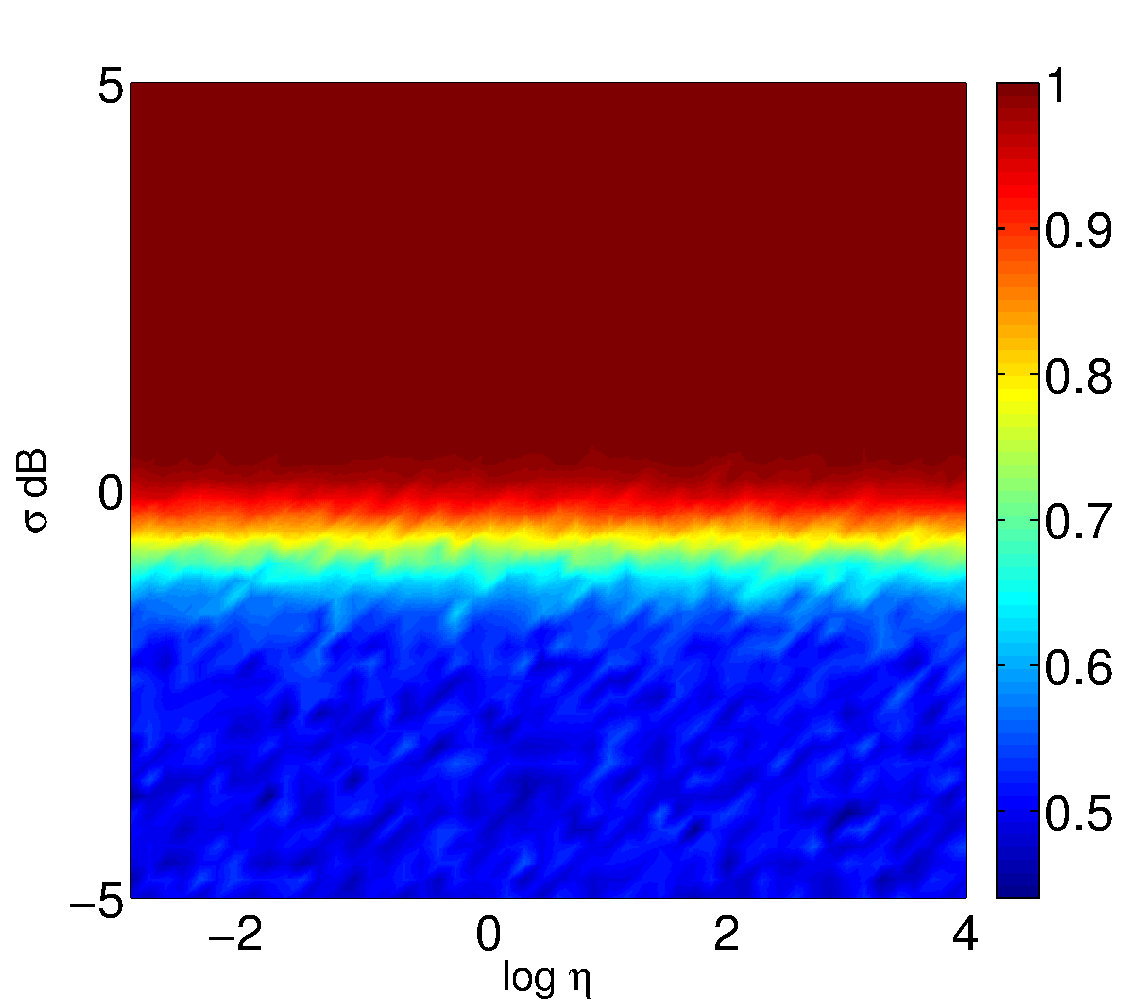
\includegraphics[width=\figwidth]{figures/ircca_auc_heatmap_n_300.pdf} 
} 
\subfigure[RCCA Difference, $n=300$]{
  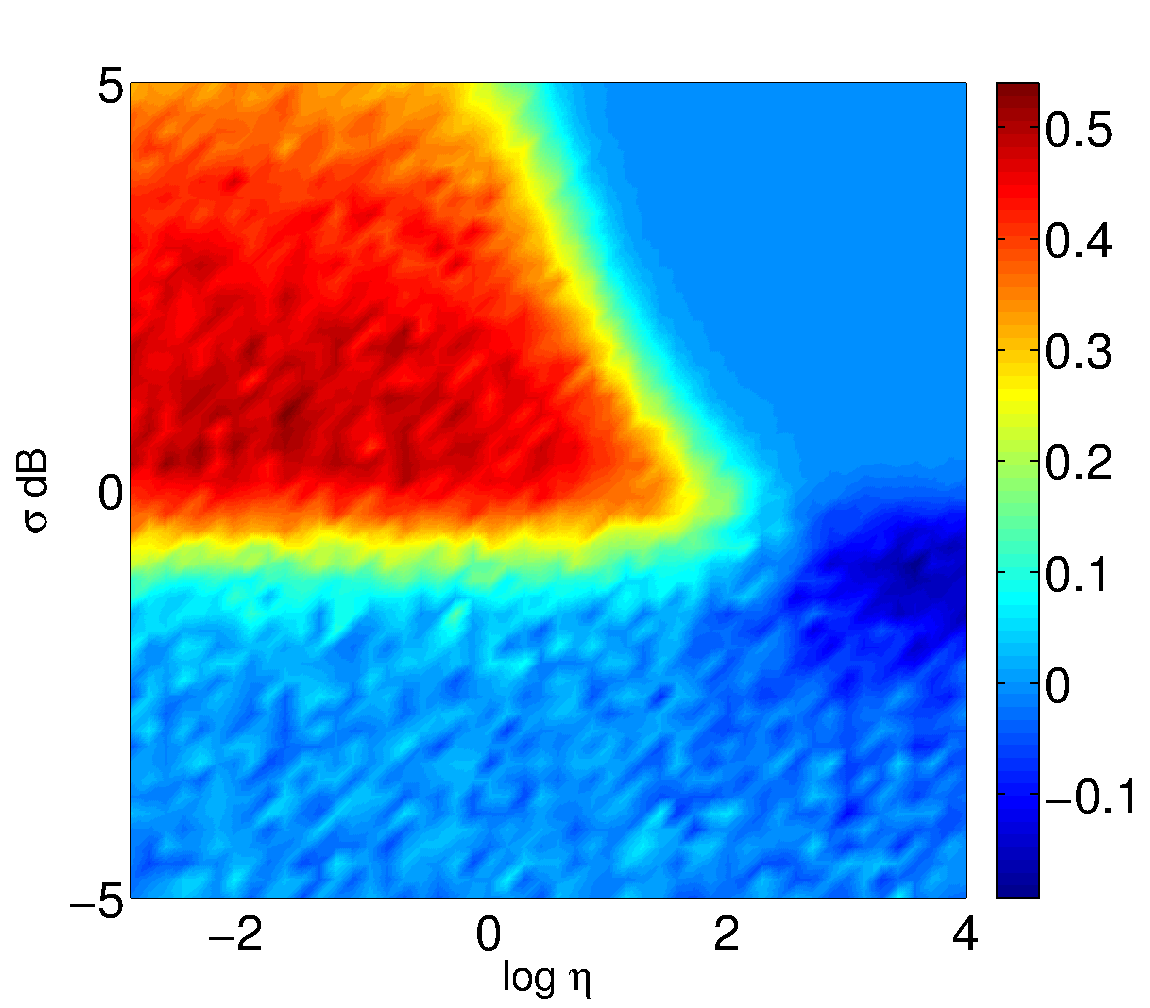
\includegraphics[width=\figwidth]{figures/ircca_auc_heatmap_diff_n_300.pdf} 
} 
\subfigure[IRCCA, $n=600$]{
  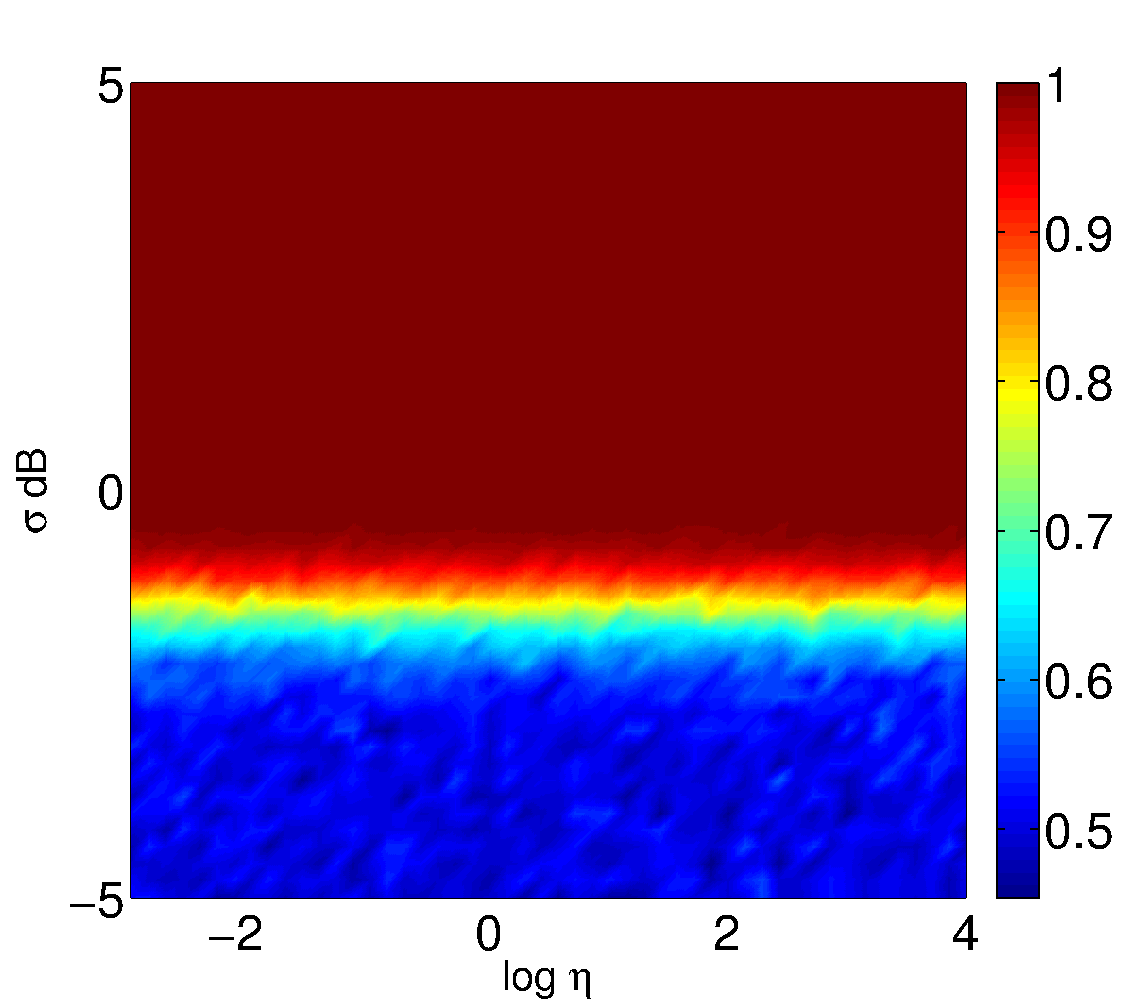
\includegraphics[width=\figwidth]{figures/ircca_auc_heatmap_n_600.pdf} 
} 
\subfigure[RCCA Difference, $n=600$]{
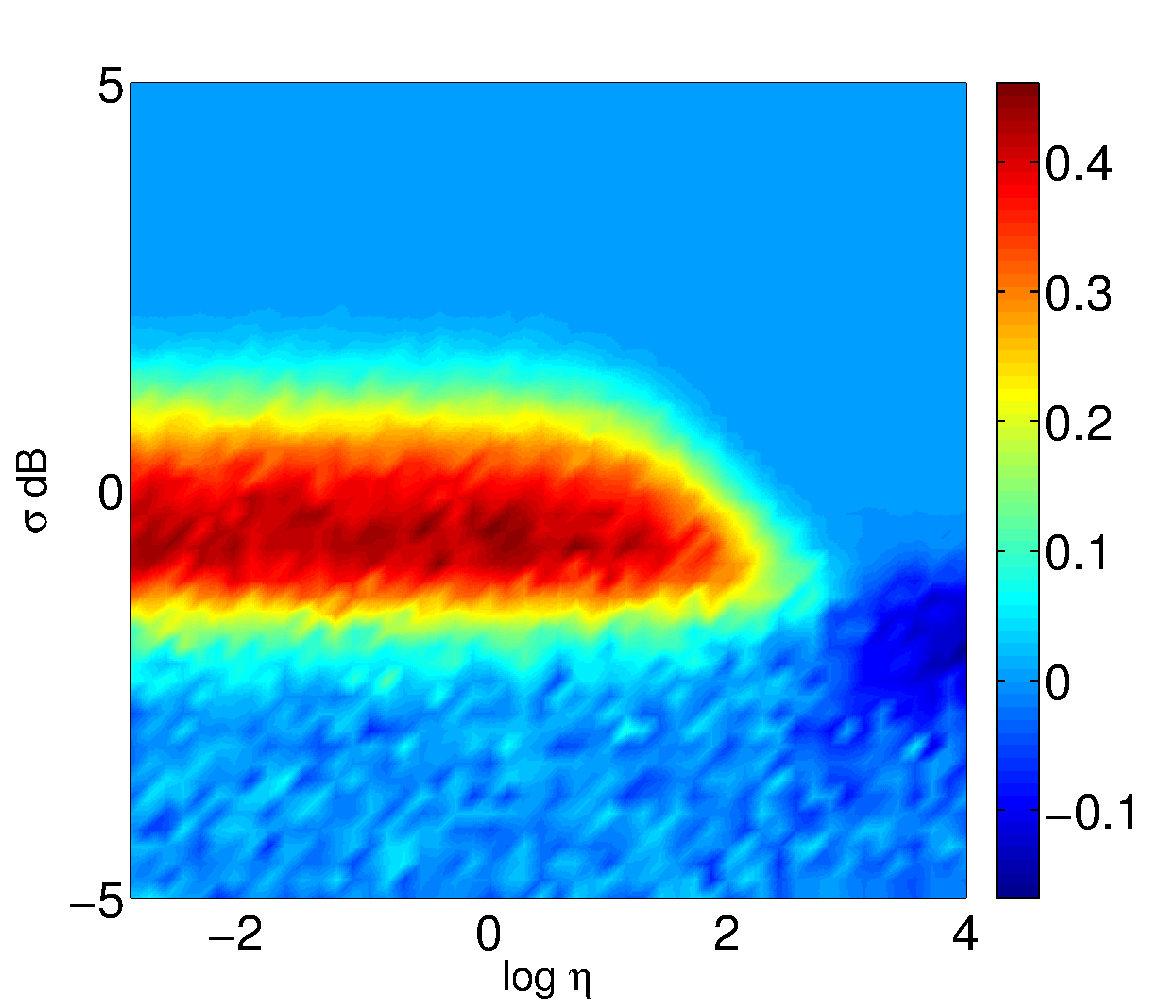
\includegraphics[width=\figwidth]{figures/ircca_auc_heatmap_diff_n_600.pdf} 
} 
\caption{Empirical AUC of the detector based on the top singular value of $\Cregtil$ in
  (\ref{eq:creghat}) based on the data models in (\ref{eq:rcca_data_model1}). Simulations
  were conducted using $d_1=200$, $d_2=150$, $\rho=0.9$, and 500 trials. Results are shown for IRCCA and
  the difference between IRCCA and RCCA for $n=300,600$. In each figure, the AUC is plotted
  for multiple combinations of $\sigma$ and $\eta$. In the difference plots, positive
  values indicate that IRCCA does better and negative values indicate that RCCA does
  better.}
\label{fig:ircca_auc_heatmap2}
\end{figure}

Figures \ref{fig:ircca_auc_heatmap1} and \ref{fig:ircca_auc_heatmap2} immediately show
that the performance of IRCCA is not affected by the regularization parameter,
$\eta$. This may be a false result because we are only considering a rank-1
signal. However, compared to the rank-1 performance of RCCA, this is a very desirable
property of IRCCA because the performance is much more predictable. Second, as the
number of training samples increases, the performance of IRCCA improves. For larger values
of $n$, IRCCA can tolerate a lower SNR, $\sigma$, and still achieve the same performance
as that of an IRCCA detector using less samples. This is a much desired improvement over
RCCA.

Comparing the difference plots between IRCCA and RCCA, we see that when $n=50$, in the
regime of medium SNR ($\sigma\approx 0$ dB) RCCA achieves better performance than
IRCCA. In the high SNR and low SNR regimes, the detectors essentially achieve the same
performance. For this value of $n$, the sample covariance matrices are ill-determined and
RCCA is necessary to prevent inverting singular matrices. It seems fitting that RCCA
achieves its best performance in this regime. 

For $n=150,300,600$, the difference plots between IRCCA and RCCA exhibit the same
behavior. For low values of $\eta$, there is a regime in which IRCCA achieves a
performance gain over RCCA. This region is quite large for $n=300$ and the performance
gain is very large for $n=300$ and $n=600$. In this low $\eta$ regime, IRCCA can achieve
the same performance as RCCA while tolerating a lower SNR. For larger values of $\eta$,
there is a regime where RCCA outperforms IRCCA. This performance gain is on the order of
0.1 AUC for all values of $n$. As previously described, we believe that in this regime of
large $\eta$, we sacrifice the accuracy of the canonical vectors and overfit the
problem. Therefore, the performance gain in this regime may not be real. Further
investigation into the accuracy of the canonical vectors of IRCCA and CCA is primary work
for the thesis.

\section{Limiting as $\eta\to\infty$}

In the previous section, the performance of RCCA improves as $\eta$ increases. This seems
contradict the notion in many regularized algorithms that over regularizing will decrease
performance. Ideally, there is an optimal regularization parameter. In this section, we let
$\eta\to\infty$ to derive a limit version of RCCA, which we call LRCCA. We compare the
performance of LRCCA to ICCA and RCCA. 

We begin with $\Creghat$ as defined in (\ref{eq:rcca_chat_decomp}). Define
$\widetilde{U}_1 = U_1(:,1:\min(d_1,n))$, $\widetilde{U}_2 = U_2(:,1:\min(d_2,n))$,
$\widetilde{V}_1 = V_1(:,1:\min(d_1,n))$, and $\widetilde{V}_2 =
V_2(:,1:\min(d_2,n))$. Then 
\begin{equation}
  \Creghat = \widetilde{U}_1\diag\left(\frac{\sigma_{1i}}{\sqrt{\sigma_{1i}^2 +
        \eta}}\right)\widetilde{V}_1^H\widetilde{V}_2
  \diag\left(\frac{\sigma_{2i}}{\sigma_{2i}^2 +\eta}\right)\widetilde{U}_2^H. 
\end{equation}
The matrix $\Creghat$ is a function of the regularization parameter, $\eta$. We would like
to examine the limiting matrix of $\Creghat$ as $\eta\to\infty$. As seen above, $\eta$
only comes into play in the two diagonal matrices and we begin by deriving the limit of
these matrices as $\eta\to\infty$. 

Clearly, as $\eta\to\infty$, these matrices become the zero matrix. However, the ratio of
the diagonal entries is what we care about. Let us consider just this.
\begin{equation*}
\lim_{\eta\to\infty} \frac{\sqrt{\frac{\sigma_{1i}^2}{\sigma_{1i}^2 +
      \eta}}}{\sqrt{\frac{\sigma_{1(i+1)}^2}{\sigma_{1(i+1)}^2 + \eta}}} =
\lim_{\eta\to\infty}
\sqrt{\frac{\sigma_{1i}^2(\sigma_{1(i+1)}^2+\eta)}{\sigma_{1(i+1)}^2(\sigma_{1i}^2 +
  \eta)} } = \frac{\sigma_{1i}}{\sigma_{1(i+1)}}
\end{equation*}
Thus, as $\eta\to\infty$, the entries along diagonal matrix approaches the ratio between
the original singular values, or a scaled version of the original singular value matrix
$\Sigma_1$ and $\Sigma_2$. As the scaling of this matrix will not affect the canonical
vectors, we can simply ignore it. Let $\widetilde{\Sigma}_1 =
\Sigma_1(1:\min(d_1,n),1:\min(d_1,n))$, and $\widetilde{\Sigma}_2 =
\Sigma_2(1:\min(d_2,n):,1:\min(d_2,n))$. Then
\begin{equation*}
  \widehat{C}_{\text{lrcca}}= \lim_{\eta\to\infty}\Creghat =
  \widetilde{U}_1\widetilde{\Sigma}_1\widetilde{V}_1^H\widetilde{V}_2\widetilde{\Sigma}_2\widetilde{U}_2^H
  = Y_1Y_2^H.
\end{equation*}
Let $\widehat{C}_{\text{lrcca}} = \widehat{F}\widehat{K}\widehat{G}^H$ be the SVD of
$\widehat{C}_{\text{lrcca}}$. Then the canonical correlation and canonical vectors are
\begin{equation}
\ba
& \widehat{\rho} = \widehat{k}_1\\
& \xIhat = f\\
& \xIIhat = g\\
\ea
\end{equation}

\section{Conclusion}

In this section, we examined the performance of regularized CCA. Regularization allows for
a tractable solution, even in the sample poor regime when the number of samples is less
than the dimension of the datasets. We first examined the behavior of the canonical
correlation coefficient estimate returned by empirical RCCA, which uses sample covariance
estimates for the unknown covariance matrices. We observed that the correlation estimate
largely affected by the choice of regularization parameter. In the case when the datasets
were generated only from Gaussian noise, RCCA sill reported a strong correlation between
the datasets. Using this correlation estimate to detect the presence of a target signal
was possible with RCCA. However, the performance of such an RCCA detector is very
irregular. The choice of $\eta$ highly affects the performance while more samples does not
necessarily lead to better detection performance. RCCA seemed to work best when used in
the sample poor regime that motivated its use. For large values of the regularization
parameter, we observed an increase in detection ability. However, evidenced by the phase
transition in the distribution of the correlation estimate, we believe this to be a
consequence of overfitting. Further work investigating the accuracy of the canonical vector
estimates is left to the thesis.

In the spirit of ICCA, we developed an informative version of RCCA called IRCCA. By
trimming the data SVDs we only use the informative components present in the data. IRCCA
exhibits some very beneficial properties. The value of the IRCCA correlation estimate
increases with the number of training samples when there is a correlated signal present
and decreases with the number of training samples when there is no correlated signal
present in the datasets. IRCCA may also be susceptible to overfitting as the correlation
estimate also exhibited a phase transition for large values of $\eta$. Using the
correlation estimate of IRCCA for signal detection provided encouraging results. The
performance of such a detector seems to be invariant to the choice of $\eta$. Unlike the
RCCA detector, the performance of IRCCA increases with an increase in the number of
training samples. Further work about the accuracy of the IRCCA canonical vectors is left
to the thesis.
